%
% Template Laporan Skripsi/Thesis 
%
% @author  Andreas Febrian, Lia Sadita 
% @version 1.03
%
% Dokumen ini dibuat berdasarkan standar IEEE dalam membuat class untuk 
% LaTeX dan konfigurasi LaTeX yang digunakan Fahrurrozi Rahman ketika 
% membuat laporan skripsi. Konfigurasi yang lama telah disesuaikan dengan 
% aturan penulisan thesis yang dikeluarkan UI pada tahun 2008.
%

%
% Tipe dokumen adalah report dengan satu kolom. 
%


\documentclass[12pt, a4paper, onecolumn, oneside, final]{report}

% Load konfigurasi LaTeX untuk tipe laporan thesis
\usepackage{_internals/uithesis}
\usepackage{alltt}
\usepackage{amsmath}

% Daftar pemenggalan suku kata dan istilah dalam LaTeX
%
% Hyphenation untuk Indonesia 
%
% @author  Andreas Febrian
% @version 1.00
% 
% Tambahkan cara pemenggalan kata-kata yang salah dipenggal secara otomatis 
% oleh LaTeX. Jika kata tersebut dapat dipenggal dengan benar, maka tidak 
% perlu ditambahkan dalam berkas ini. Tanda pemenggalan kata menggunakan 
% tanda '-'; contoh:
% menarik
%   --> pemenggalan: me-na-rik
%

\hyphenation{
    % alphabhet A
    a-na-li-sa a-tur 
    a-pli-ka-si 
    % alphabhet B
    ba-ngun-an 
    be-be-ra-pa 
    ber-ge-rak
    ber-ke-lan-jut-an 
    ber-pe-nga-ruh 
    % alphabhet C
    ca-ri
    % alphabhet D
    di-sim-pan di-pim-pin de-ngan da-e-rah di-ba-ngun da-pat di-nya-ta-kan 
    di-sim-bol-kan di-pi-lih di-li-hat de-fi-ni-si
    % alphabhet E
    e-ner-gi eks-klu-sif
    % alphabhet F
    fa-si-li-tas
    % alphabhet G
    ga-bung-an ge-rak
    % alphabhet H
    ha-lang-an
    % alphabhet I
    % alphabhet J
    % alphabhet K
    ke-hi-lang-an
    ku-ning 
    kua-li-tas ka-me-ra ke-mung-kin-an ke-se-pa-ham-an
    % alphabhet L
    ling-kung-an
    % alphabhet M
    me-neng-ah
    meng-a-tas-i me-mung-kin-kan me-nge-na-i me-ngi-rim-kan 
    meng-u-bah meng-a-dap-ta-si me-nya-ta-kan mo-di-fi-ka-si
    meng-a-tur
    % alphabhet N
    nya-ta non-eks-klu-sif
    % alphabhet O
    % alphabhet P
	pe-nye-rap-an 
	pe-ngon-trol
    pe-mo-del-an
    pe-ran  pe-ran-an-nya
    pem-ba-ngun-an pre-si-den pe-me-rin-tah prio-ri-tas peng-am-bil-an 
    peng-ga-bung-an pe-nga-was-an pe-ngem-bang-an 
    pe-nga-ruh pa-ra-lel-is-me per-hi-tung-an per-ma-sa-lah-an 
    pen-ca-ri-an peng-struk-tur-an
    % alphabhet Q
    % alphabhet R
    ran-cang-an
    % alphabhet S
    si-mu-la-si sa-ngat
    % alphabhet T
    te-ngah
    ter-da-pat
    % alphabhet U
    % alphabhet V
    % alphabhet W
    % alphabhet X
    % alphabhet Y
    % alphabhet Z
    % special
}

% Load konfigurasi khusus untuk laporan yang sedang dibuat
%-----------------------------------------------------------------------------%
% Informasi Mengenai Dokumen
%-----------------------------------------------------------------------------%
% 
% Judul laporan. 
\var{\judul}{Analisis Kinerja Tuning Hypervisor KVM dengan \f{CloudStack Agent} pada Lingkungan \f{Virtual Machine} di \f{Cloud Management Platform} Apache CloudStack}
% 
% Tulis kembali judul laporan, kali ini akan diubah menjadi huruf kapital
\Var{\Judul}{Analisis Kinerja Tuning Hypervisor KVM dengan \f{Cloudstack Agent} pada Lingkungan \f{Virtual Machine} di \f{Cloud Management Platform } Apache CloudStack}
% 
% Tulis kembali judul laporan namun dengan bahasa Ingris
\var{\judulInggris}{Performance Analysis of KVM Hypervisor Tuning with CloudStack Agent for Virtual Machine Environment on Cloud Management Platform Apache CloudStack}

% 
% Tipe laporan, dapat berisi Skripsi, Tugas Akhir, Thesis, atau Disertasi
\var{\type}{Skripsi}
% 
% Tulis kembali tipe laporan, kali ini akan diubah menjadi huruf kapital
\Var{\Type}{Skripsi}
% 
% Tulis nama penulis 
\var{\penulis}{Ariq Pradipa Santoso}
% 
% Tulis kembali nama penulis, kali ini akan diubah menjadi huruf kapital
\Var{\Penulis}{Ariq Pradipa Santoso}
% 
% Tulis NPM penulis
\var{\npm}{2006527052}
% 
% Tuliskan Fakultas dimana penulis berada
\Var{\Fakultas}{Teknik}
\var{\fakultas}{Teknik}
% 
% Tuliskan Program Studi yang diambil penulis
\Var{\Program}{Teknik Komputer}
\var{\program}{Teknik Komputer}
% 
% Tuliskan tahun publikasi laporan
\Var{\bulan}{Juni}
\Var{\tahun}{2024}
% 
% Tuliskan gelar yang akan diperoleh dengan menyerahkan laporan ini
\var{\gelar}{Sarjana Teknik}
% 
% Tuliskan tanggal pengesahan laporan, waktu dimana laporan diserahkan ke 
% penguji/sekretariat
\var{\tanggalPengesahan}{Juni 2024}
% 
% Tuliskan tanggal keputusan sidang dikeluarkan dan penulis dinyatakan 
% lulus/tidak lulus
\var{\tanggalLulus}{Juni 2024}
% 
% Tuliskan pembimbing 
\var{\pembimbing}{Yan Maraden S.T., M.T.}
% 
% Tuliskan penguji
\var{\pengujisatu}{Dr. Ruki Harwahyu, ST. MT. MSc.}
\var{\pengujidua}{I Gde Dharma Nugraha, S.T., M.T., Ph.D}
% 
% Alias untuk memudahkan alur penulisan paa saat menulis laporan
\var{\saya}{Penulis}

%-----------------------------------------------------------------------------%
% Judul Setiap Bab
%-----------------------------------------------------------------------------%
% 
% Berikut ada judul-judul setiap bab. 
% Silahkan diubah sesuai dengan kebutuhan. 
% 
\Var{\kataPengantar}{Kata Pengantar}
\Var{\babSatu}{Pendahuluan}
\Var{\babDua}{Tuning Hypervisor KVM}
\Var{\babTiga}{Metode Pengujian Tuning Parametr Hypervisor KVM dengan Cloudstack Agent}
\Var{\babEmpat}{Hasil Pengujian Tuning Parameter Hypervisor KVM dengan Cloudstack Agent}
\Var{\babLima}{Kesimpulan}
% \Var{\babEnam}{Bab Enam}
% \Var{\kesimpulan}{Kesimpulan dan Saran}


% Daftar istilah yang mungkin perlu ditandai 
%
% @author  Andreas Febrian
% @version 1.00
% 
% Mendaftar seluruh istilah yang mungkin akan perlu dijadikan 
% italic atau bold pada setiap kemunculannya dalam dokumen. 
% 

\var{\license}{\f{Creative Common License 1.0 Generic}}
\var{\bslash}{$\setminus$}

\var{\cc}{\f{Cloud Computing}}
\var{\vm}{\f{Virtual Machine}}
\var{\vmm}{\f{Virtual Machine Monitor}}
\var{\oss}{\f{open source}}
\var{\ssim}{\f{Structural Similarity Index Measure}}


% Awal bagian penulisan laporan
\begin{document}
%
% Sampul Laporan
%
% Sampul Laporan

%
% @author  unknown
% @version 1.01
% @edit by Andreas Febrian
%

\begin{titlepage}
    \begin{center}    
        \begin{figure}
            \begin{center}
                
\includegraphics[width=2.5cm]{_internals/makara.eps}
            \end{center}
        \end{figure}    
        \vspace*{0cm}
        \bo{
        	UNIVERSITAS INDONESIA\\
        }
        
        \vspace*{1.0cm}
        % judul thesis harus dalam 14pt Times New Roman
        \bo{\Judul} \\[1.0cm]

        \vspace*{2.5 cm}    
        % harus dalam 14pt Times New Roman
        \bo{\Type}

        \vspace*{3 cm}       
        % penulis dan npm
        \bo{\Penulis} \\
        \bo{\npm} \\

        \vspace*{5.0cm}

        % informasi mengenai fakultas dan program studi
        \bo{
        	FAKULTAS \Fakultas\\
        	PROGRAM STUDI \Program \\
        	DEPOK \\
        	\tahun
        }
    \end{center}
\end{titlepage}


%
% Gunakan penomeran romawi
\pagenumbering{roman}

%
% load halaman judul dalam
\addChapter{HALAMAN JUDUL}
%
% Halaman Judul Laporan 
%
% @author  unknown
% @version 1.01
% @edit by Andreas Febrian
%


\begin{titlepage}
    \begin{center}\begin{figure}
            \begin{center}
                
\includegraphics[width=2.5cm]{_internals/makara.eps}
            \end{center}
        \end{figure}    
        \vspace*{0cm}
        \bo{
        	UNIVERSITAS INDONESIA\\
        }
        
        \vspace*{1.0cm}
        % judul thesis harus dalam 14pt Times New Roman
        \bo{\Judul} \\[1.0cm]

        \vspace*{2.5 cm}    
        % harus dalam 14pt Times New Roman
        \bo{\Type} \\
        % keterangan prasyarat
        \bo{Diajukan sebagai salah satu syarat untuk memperoleh gelar \\
        \gelar}\\

        \vspace*{3 cm}       
        % penulis dan npm
        \bo{\Penulis} \\
        \bo{\npm} \\

        \vspace*{5.0cm}

        % informasi mengenai fakultas dan program studi
        \bo{
        	FAKULTAS \Fakultas\\
        	PROGRAM STUDI \Program \\
        	DEPOK \\
        	\bulan\ \tahun
        }
    \end{center}
\end{titlepage}

%
% setelah bagian ini, halaman dihitung sebagai halaman ke 2
\setcounter{page}{2}

%
% load halaman pengesahan
\addChapter{LEMBAR PERSETUJUAN}
%
% Halaman Pengesahan
%
% @author  Andreas Febrian
% @version 1.01
%

\chapter*{HALAMAN PERSETUJUAN}

\vspace*{0.2cm}
\noindent 

\noindent
\begin{tabular}{l l p{11cm}}
	\bo{Judul}&: & \judul \\ 
	\bo{Nama}&: & \penulis \\
	\bo{NPM}&: & \npm \\
\end{tabular} \\

\vspace*{1.2cm}

\noindent Laporan \type~ini telah diperiksa dan disetujui.\\[0.3cm]
\begin{center}
\tanggalPengesahan \\[2cm]


\underline{\pembimbing}\\[0.1cm]
Pembimbing \type
\end{center}

\newpage
%
% load halaman orisinalitas 
\addChapter{LEMBAR PERNYATAAN ORISINALITAS}
%
% Halaman Orisinalitas
%
% @author  Andreas Febrian
% @version 1.01
%

\chapter*{Halaman Pernyataan Orisinalitas}
\vspace*{2cm}

\begin{center}
	\bo{\type~ini adalah hasil karya saya sendiri, \\ 
	dan semua sumber baik yang dikutip maupun dirujuk \\
	telah saya nyatakan dengan benar.} \\
	\vspace*{2.6cm}
	
	\begin{tabular}{l c l}
	\bo{Nama} & : & \bo{\penulis} \\
	\bo{NPM} & : & \bo{\npm} \\ 
	\bo{Tanda Tangan} & : & \\
	& & \\
	& & \\
	\bo{Tanggal} & : & \bo{\tanggalPengesahan} \\	
	\end{tabular}
\end{center}

\newpage
%
%
\addChapter{LEMBAR PENGESAHAN}
%
% Halaman Pengesahan Sidang
%
% @author  Andreas Febrian, Andre Tampubolon 
% @version 1.02
%

\chapter*{HALAMAN PENGESAHAN}

\vspace*{0.4cm}
\noindent

\noindent
\begin{tabular}{ll p{9cm}}
	\type~ini diajukan oleh & : &          \\
	Nama                    & : & \penulis \\
	NPM                     & : & \npm     \\
	Program Studi           & : & \program \\
	Judul \type             & : & \judul   \\
\end{tabular} \\

\vspace*{1.0cm}

\noindent \bo{Telah berhasil dipertahankan di hadapan Dewan Penguji
	dan diterima sebagai bagian persyaratan yang diperlukan untuk
	memperoleh gelar \gelar~pada Program Studi \program, Fakultas
	\fakultas, Universitas Indonesia.}\\[0.2cm]

\begin{center}
	\bo{DEWAN PENGUJI}
\end{center}

\vspace*{0.3cm}

\begin{tabular}{l l l l }
	           &   &              &                   \\
	Pembimbing & : & \pembimbing  & (\hspace*{3.0cm}) \\
	           &   &              &                   \\
	Penguji    & : & \pengujisatu & (\hspace*{3.0cm}) \\
	           &   &              &                   \\
	Penguji    & : & \pengujidua  & (\hspace*{3.0cm}) \\
\end{tabular}\\

%\todo{Jangan lupa mengisi nama para penguji.}

\vspace*{2.0cm}

\begin{tabular}{ll l}
	Ditetapkan di & : & Depok         \\
	Tanggal       & : & \tanggalLulus \\
\end{tabular}


\newpage
%
%
\addChapter{\kataPengantar}
%-----------------------------------------------------------------------------%
\chapter*{Kata Pengantar}
%-----------------------------------------------------------------------------%
Dengan mengucap syukur kehadirat Allah SWT, saya dapat menyelesaikan skripsi ini sebagai salah satu syarat untuk menyelesaikan program studi Teknik Komputer di Universitas Indonesia. Penulisan skripsi ini tidak lepas dari dukungan dan bantuan berbagai pihak, yang dengan tulus saya ucapkan terima kasih.

Ucapan terima kasih yang sebesar-besarnya saya persembahkan kepada kedua orang tua saya, yang telah memberikan doa, dukungan moral, dan finansial selama proses pembuatan skripsi ini. Tak lupa kepada dosen pembimbing, Bapak Yan Maraden, S.T., M.T. atas bimbingan, arahan, dan kritik yang membangun selama proses penulisan skripsi ini.

Saya juga ingin mengucapkan terima kasih kepada teman-teman di Teknik Komputer Universitas Indonesia dan Maritsa Putriniandi Az-Zahra yang telah memberikan semangat dan dukungan selama pengerjaan skripsi. Pengalaman dan ilmu yang saya peroleh selama proses pembelajaran di universitas ini sangat berharga dan menjadi motivasi dalam penyelesaian skripsi ini.

Skripsi ini berjudul \judul yang merupakan upaya saya untuk memberikan kontribusi dalam bidang cloud serta sebagai aplikasi dari teori yang telah saya pelajari. Saya berharap skripsi ini dapat bermanfaat bagi pengembangan ilmu pengetahuan, khususnya bagi para peneliti dan mahasiswa yang berkecimpung dalam bidang yang sama.

Akhir kata, semoga skripsi ini dapat memberikan manfaat dan inspirasi bagi kita semua. Kritik dan saran yang membangun selalu saya harapkan untuk perbaikan di masa yang akan datang.


\vspace*{0.1cm}
\begin{flushright}
	Depok, 31 Mei 2024\\[0.1cm]
	\vspace*{1cm}
	\penulis

\end{flushright}
%
%
\addChapter{LEMBAR PERSETUJUAN PUBLIKASI ILMIAH}
% 
% @author  Andre Tampubolon, Andreas Febrian
% @version 1.01
% 

\chapter*{Halaman Pernyataan Persetujuan Publikasi Tugas Akhir untuk Kepentingan Akademis}

\vspace*{0.2cm}
\noindent
Sebagai sivitas akademik Universitas Indonesia, saya yang bertanda
tangan di bawah ini:
\vspace*{0.4cm}


\begin{tabular}{p{4.2cm} l p{6cm}}
	\bo{Nama}          & : & \penulis  \\
	\bo{NPM}           & : & \npm      \\
	\bo{Program Studi} & : & \program  \\
	\bo{Fakultas}      & : & \fakultas \\
	\bo{Jenis Karya}   & : & \type     \\
\end{tabular}

\vspace*{0.6cm}
\noindent demi pengembangan ilmu pengetahuan, menyetujui untuk memberikan
kepada Universitas Indonesia \bo{Hak Bebas Royalti Noneksklusif
	(\textit{Non-exclusive Royalty Free Right})} atas karya ilmiah saya yang berjudul:
\begin{center}
	\judul
\end{center}
beserta perangkat yang ada (jika diperlukan). Dengan Hak Bebas Royalti
Noneksklusif ini Universitas Indonesia berhak menyimpan,
mengalihmedia/formatkan, mengelola dalam bentuk pangkalan data
(\textit{database}), merawat, dan memublikasikan tugas akhir saya selama
tetap mencantumkan nama saya sebagai penulis/pencipta dan sebagai
pemilik Hak Cipta. \\

\noindent Demikian pernyatan ini saya buat dengan sebenarnya.

\begin{center}
	\vspace*{0.8cm}
	\begin{tabular}{rl}
		Dibuat di :    & Depok              \\
		Pada tanggal : & \tanggalPengesahan \\
	\end{tabular}\\

	\vspace*{0.2cm}
	Yang menyatakan \\
	\vspace*{1.1cm}
	(\penulis)
\end{center}

\newpage


%
% 
\addChapter{ABSTRAK}
%
% Halaman Abstrak
%
% @author  Andreas Febrian
% @version 1.00
%

\chapter*{Abstrak}

\vspace*{0.2cm}
{
	\setlength{\parindent}{0pt}

	\begin{tabular}{@{}l l p{10cm}}
		Nama          & : & \penulis    \\
		Program Studi & : & \program    \\
		Judul         & : & \judul      \\
		Pembimbing    & : & \pembimbing \\
	\end{tabular}

	\bigskip
	\bigskip

	\cc\ menyediakan akses mudah ke berbagai sumber daya melalui jaringan internet, dengan jangkauan jaringan yang luas, kemampuan elastisitas yang cepat, dan layanan yang dapat diukur. Dalam penelitian ini, digunakan \f{Cloud Management Platform} Apache CloudStack untuk membangun sistem Cloud sendiri. Sistem ini menggunakan sistem operasi Ubuntu dan hypervisor KVM (Kernel-based Virtual Machine) untuk menguji performa dan optimalisasi konfigurasi hypervisor dalam menjalankan tugas-tugas komputasi tertentu.

	Penelitian ini bertujuan untuk menganalisis apakah konfigurasi default dari hypervisor KVM sudah optimal dan bagaimana konfigurasi hypervisor KVM dapat meningkatkan performa dalam menjalankan tugas komputasi seperti kompresi video, enkripsi, dekripsi, dan validasi integritas data. Metode yang digunakan melibatkan pengujian performa hypervisor KVM dengan melakukan berbagai tugas komputasi dan mengukur waktu yang diperlukan untuk menyelesaikan tugas-tugas tersebut. Hasil pengujian menunjukkan bahwa konfigurasi hypervisor dengan menambahkan flag tertentu seperti SSSE3, SSE4.1, SSE4.2, SSE4a, dan AES dapat meningkatkan performa komputasi secara signifikan.

	Kesimpulan dari penelitian ini adalah bahwa konfigurasi default hypervisor KVM bersifat minimal dan perlu dilakukan konfigurasi untuk mencapai performa optimal. Konfigurasi hypervisor yang tepat dapat mempercepat kompresi video hingga 2.4 kali, validasi integritas data hingga 7.56 kali, enkripsi AES hingga 2.1 kali, dan dekripsi AES hingga 2.68 kali dibandingkan dengan konfigurasi default. Penelitian ini diharapkan memberikan kontribusi akademis dalam bidang optimalisasi infrastruktur cloud.

	\bigskip

	Kata kunci:\\
	Cloud Computing, KVM Hypervisor, Optimisasi Performa, Apache CloudStack
}

\newpage
%
%
%
% Halaman Abstract
%
% @author  Andreas Febrian
% @version 1.00
%

\chapter*{Abstract}

\vspace*{0.2cm}
{
	\setlength{\parindent}{0pt}
	
	\begin{tabular}{@{}l l p{10cm}}
		Name&: & \penulis \\
		Study Program&: & \program \\
		Title&: & \judulInggris \\
		Counsellor&: & \pembimbing \\
	\end{tabular}

	\bigskip
	\bigskip

	Cloud Computing provides easy access to various resources over the internet, with a wide network reach, fast elasticity capabilities, and measurable services. In this research, the Apache CloudStack Cloud Management Platform is utilized to build a Cloud system. This system uses the Ubuntu operating system and KVM (Kernel-based Virtual Machine) hypervisor to test performance and optimize the hypervisor configuration for specific computing tasks.
	
	The aim of this research is to analyze whether the default configuration of the KVM hypervisor is optimal and how tuning the KVM hypervisor can enhance performance in executing computing tasks such as video compression, encryption, decryption, and data integrity validation. The methodology involves performance testing of the KVM hypervisor by executing various computing tasks and measuring the time taken to complete these tasks. The test results indicate that tuning the hypervisor by adding specific flags such as SSSE3, SSE4.1, SSE4.2, SSE4a, and AES can significantly improve computational performance.
	
	The conclusion drawn from this research is that the default configuration of the KVM hypervisor is minimal and requires tuning to achieve optimal performance. Proper hypervisor tuning can accelerate video compression by up to 2.4 times, data integrity validation by up to 7.56 times, AES encryption by up to 2.1 times, and AES decryption by up to 2.68 times compared to the default configuration. This research is expected to make an academic contribution in the field of cloud infrastructure optimization.

	\bigskip

	Key words:\\
	Cloud Computing, KVM Hypervisor, Performance Optimization, Apache CloudStack
}

\newpage

%
% Daftar isi, gambar, dan tabel
%
\phantomsection
\tableofcontents
\clearpage
\phantomsection
\listoffigures
\clearpage
\phantomsection
\listoftables
\clearpage
\phantomsection
\listoflistings
\clearpage

%
% Gunakan penomeran Arab (1, 2, 3, ...) setelah bagian ini.
%
\pagenumbering{arabic}

%
%
%
%-----------------------------------------------------------------------------%
\chapter{\babSatu}
%-----------------------------------------------------------------------------%
% \todo{tambahkan kata-kata pengantar bab 1 disini}


%-----------------------------------------------------------------------------%
\section{Latar Belakang}
%-----------------------------------------------------------------------------%
\cc\ adalah sebuah sistem informasi yang menyediakan akses mudah ke berbagai komponen sumber daya, seperti server, aplikasi, dan database, melalui jaringan internet. Dalam sistem ini, sumber daya disimpan dan dikelola di pusat data yang terhubung dengan internet. \cc\ memiliki beberapa karakteristik utama, yakni layanan \f{on-demand}, akses jaringan yang luas, elastisitas yang cepat, dan layanan yang terukur. Terdapat tiga model layanan pada \cc, yaitu \f{Software as a Service} (SaaS), \f{Platform as a Service} (PaaS), dan Infrastructure as a Service (IaaS). Dan juga terdapat empat model implementasi pada \cc, yaitu \f{private cloud, community cloud, public cloud,} dan \f{hybrid cloud,} masing-masing sesuai dengan kebutuhan dan kegunaan dari pengguna yang berbeda \cite{mell2009nist}.

Pengguna dapat membuat sistem \cc nya sendiri dengan menggunakan \f{Cloud Management Platform} Apache CloudStack. Apache CloudStack adalah perangkat lunak \oss\ yang dirancang untuk implementasi dan administrasi jaringan \vm. CloudStack berfungsi sebagai platform \cc\ Infrastructure as a Service (IaaS) yang \f{reliable}, Apache CloudStack juga dikenal karena kemampuan \f{high availability} dan skalabilitasnya. Apache CloudStack digunakan oleh berbagai penyedia layanan cloud untuk menyediakan layanan cloud publik, CloudStack juga digunakan oleh banyak perusahaan untuk membentuk solusi \f{private cloud} atau sebagai bagian dari konfigurasi \f{hybrid cloud} \cite{cloudstackabout}.

Untuk menjalankan Apache Cloudstack diperlukan sebuah hypervisor. Hypervisor atau biasa juga dikenal sebagai \f{Virtual Machine Monitor} adalah komponen virtualisasi yang mengawasi dan mengelola sistem operasi \f{guest} pada sistem \f{host} \cite{scarfone2009nist}. Hypervisor mengontrol komunikasi instruksi antara sistem operasi \f{guest} dan \f{hardware} dari \f{host} \cite{scarfone2009nist}.

Penggunaan KVM sebagai hypervisor untuk menjalankan \vm\ pada Apache Cloudstack telah menjadi praktik umum. Hypervisor KVM \f{(Kernel-based Virtual Machine)} adalah sebuah hypervisor berbasis kernel yang memungkinkan virtualisasi pada sistem operasi Linux \cite{whatiskvm}. KVM memanfaatkan modul kernel untuk menyediakan dukungan langsung untuk virtualisasi dengan menggunakan instruksi \f{hardware} yang mendukung teknologi virtualisasi, seperti Intel VT atau AMD-V. Namun, pertanyaan mendasar muncul: apakah hypervisor ini telah dikonfigurasi secara optimal untuk menjalankan \vm\ dan mengerjakan tugas yang diberikan dengan baik? Penelitian ini bertujuan untuk menganalisis apakah konfigurasi hypervisor KVM telah diatur dengan tepat dan baik. Pada penelitian ini, \saya\ akan menguji performa hypervisor dengan melakukan beberapa tugas komputasi, seperti kompresi video \cite{Folgar2014eg}, enkripsi, dekripsi, dan juga validasi integritas data. Selanjutnya, waktu yang diperlukan untuk menyelesaikan proses komputasi ini akan diukur dan dibandingkan dalam rangka evaluasi performa.


%-----------------------------------------------------------------------------%
\section{Permasalahan}
%-----------------------------------------------------------------------------%
Pada bagian ini akan dijelaskan mengenai definisi permasalahan yang \saya\ hadapi dan ingin diselesaikan serta asumsi dan batasan yang digunakan dalam menyelesaikannya.

%-----------------------------------------------------------------------------%
\subsection{Definisi Permasalahan}
%-----------------------------------------------------------------------------%
Berdasarkan latar belakang yang telah dijelaskan pada bab 1.1, bahasan definisi permasalahan yang akan dibahas pada penelitian ini adalah sebagai berikut:
\begin{enumerate}
      \item Apakah konfigurasi default dari Hypervisor KVM sudah dibuat dengan optimal?
      \item Apakah tuning Hypervisor KVM untuk \vm\ di Apache Cloudstack memberikan efek yang signifikan terhadap performa tugas komputasi seperti kompresi video, enkripsi dan dekripsi AES, dan validasi integritas data dengan CRC32?
      \item Bagaimana konfigurasi Hypervisor KVM dapat diatur secara optimal untuk meningkatkan efisiensi atau kecepatan dalam menangani tugas komputasi tertentu pada Apache CloudStack?
\end{enumerate}

%-----------------------------------------------------------------------------%
\subsection{Batasan Permasalahan}
%-----------------------------------------------------------------------------%
Karena berbagai kendala yang dihadapi pada skripsi ini dilakukan pembatasan masalah pada penelitian  sebagai berikut:
\begin{enumerate}
      \item Penelitian dilakukan menggunakan perangkat laptop dengan spesifikasi sebagai berikut:
            \begin{itemize}
                  \item CPU: AMD Ryzen 7 4800H x64.
                  \item RAM: 16 GB.
                  \item Penyimpanan: 1TB pada SSD.
            \end{itemize}
      \item Sistem operasi yang digunakan adalah Ubuntu Server 22.04 LTS.
      \item Karena perangkat menggunakan CPU AMD, implementasi teknologi virtualisasi yang diadopsi adalah AMD-V.
      \item Parameter yang menjadi fokus analisis dalam penelitian ini adalah waktu kompresi video, waktu enkrispsi dan dekripsi dengan AES, dan waktu validasi integritas data dengan CRC32 antara hypervisor default dan hypervisor yang telah dituning.
\end{enumerate}


%-----------------------------------------------------------------------------%
\section{Tujuan}
%-----------------------------------------------------------------------------%
Penelitian ini berfokus pada analisis performa dari tuning Hypervirsor KVM dengan menggunkaan CloudStack Agent pada \f{Cloud Management Platform} Apache CloudStack. Dengan tujuan sebagai berikut:

\begin{enumerate}
      \item  Memahami efek dari tuning hypervisor KVM pada virtual machine di lingkungan Apache CloudStack terhadap performa tugas komputasi seperti kompresi video, enkripsi dan dekripsi AES, dan validasi integritas data dengan CRC32.

      \item Menemukan metodologi tuning hypervisor KVM yang optimal untuk meningkatkan efisiensi atau kecepatan dalam menangani tugas komputasi tertentu pada Apache CloudStack.

\end{enumerate}

Hasil penelitian ini diharapkan tidak hanya memberikan panduan praktis tetapi juga kontribusi akademis dalam bidang optimalisasi infrastruktur cloud.

%-----------------------------------------------------------------------------%
\section{Metodologi Penelitian}
%-----------------------------------------------------------------------------%
Beberapa metodologi yang dilakukan pada penelitian ini, antara lain:
\begin{enumerate}
      \item Studi Literatur

            Studi literatur dalam penelitian ini dilakukan dengan melakukan pencarian, membaca, dan memahami jurnal serta sumber referensi yang terkait dengan \cc. Penelitian ini juga melibatkan eksplorasi literatur yang mendalam terkait dengan metode tuning hypervisor KVM, kondisi saat melakukan pemrosesan kompresi video, enkripsi dan dekripsi AES, dan juga mengenai validasi integritas data dengan CRC32 serta evaluasi keuntungan dan kerugian yang mungkin muncul akibat hasil tuning ini.

      \item Pengumpulan Data

            Pada penelitian ini, akan dilakukan tiga pengujian
            \begin{enumerate}
                  \item Kompresi Video

                        Kompresi video akan dilakukan menggunakan ffmpeg pada dua sistem, yaitu sistem yang menggunakan KVM default dan sistem yang menggunakan KVM yang sudah dituning. Pada masing-masing sistem, kompresi video akan dilakukan sebanyak 100 kali. Setelah itu, waktu rata-rata kompresi video pada kedua sistem akan dibandingkan dan dianalisis.

                  \item Validasi Integritas Data CRC32

                        Validasi Integritas Data dengan menggunakan fungsi CRC32 akan dilakukan dengan program benchmark yang dibuat \saya\ dengan python pada kedua sistem. Pada masing-masing sistem, validasi CRC32 akan dilakukan sebanyak 100 kali. Setelah itu, waktu rata-rata validasi integritas data dengan CRC32 pada kedua sistem akan dibandingkan dan dianalisis.

                  \item Enkripsi dan Dekripsi AES

                        Enkripsi dan dekripsi AES akan dilakukan dengan program benchmark yang dibuat \saya\ dengan python pada kedua sistem. Pada masing-masing sistem, enkripsi dan dekripsis AES akan dilakukan sebanyak 100 kali. Setelah itu, waktu rata-rata enkripsi dan dekripsi AES pada kedua sistem akan dibandingkan dan dianalisis.
            \end{enumerate}

      \item Analisis

            Setelah itu, dilakukan evaluasi terhadap hasil yang diperoleh dan kemudian menyusun kesimpulan.
\end{enumerate}


%-----------------------------------------------------------------------------%
\section{Sistematika Penulisan}
%-----------------------------------------------------------------------------%
Pada penulisan skripsi ini terdiri dari 5 bab dengan pokok bahasan yang berbeda-beda untuk setiap bab.
\begin{itemize}
      \item BAB I PENDAHULUAN

            Bab I membahas tentang pendahuluan penelitian, yang meliputi latar belakang masalah, rumusan masalah, batasan masalah, tujuan penelitian, metode penelitian, dan sistematika penulisan.

      \item BAB II TUNING HYPERVISOR KVM

            Bab II membahas tentang landasan teori yang digunakan untuk memahami dan menganalisis hasil penelitian.

      \item BAB III METODE PENGUJIAN TUNING PARAMETER HYPERVISOR KVM DENGAN CLOUDSTACK AGENT

            Bab III membahas tentang tahapan dan bagaimana metode yang digunakan untuk melakukan tuning dan pengujian dari tuning parameter Hypervisor KVM, dan juga bagaimana analisis akan dilakukan.

      \item BAB IV HASIL PENGUJIAN TUNING PARAMETER HYPERVISOR KVM DENGAN CLOUDSTACK AGENT

            Bab IV menjelaskan hasil penelitian yang terdiri dari pengujian tuning parameter hypervisor KVM, dan dilakukan analisis performa hypervisor KVM setelah proses tuning.

      \item BAB V PENUTUP

            Bab V menjelaskan kesimpulan dari penelitian dilakukan dan saran.
\end{itemize}
%-----------------------------------------------------------------------------%
\chapter{\babDua}
%-----------------------------------------------------------------------------%

Pada bab ini, akan dijelaskan mengenai landasan teori yang menjadi dasar untuk memahami, menganalisis, dan menyelesaikan permasalahan yang menjadi fokus penelitian ini.

%-----------------------------------------------------------------------------%
\section{\cc}
%-----------------------------------------------------------------------------%
\cc, menurut definisi National Institute of Standards and Technology (NIST), merupakan suatu model komputasi yang menyediakan akses dan konfigurasi sumber daya komputasi seperti jaringan, server, penyimpanan, aplikasi, dan layanan secara on-demand, memungkinkan pelepasan yang cepat tanpa interaksi yang kompleks dengan penyedia layanan\cite{mell2009nist}. \cc\ bukanlah suatu teknologi spesifik, melainkan sebuah model yang menggambarkan operasional dan ekonomi untuk penyediaan serta penggunaan infrastruktur IT dan layanan terkait. Beberapa definisi cloud memiliki karakteristik umum yang sama, seperti \f{pay-per-use} (pembayaran sesuai dengan penggunaan), kapasitas yang elastis, layanan mandiri, dan abstraksi atau virtualisasi sumber daya\cite{Buyya_Broberg_Goscinski_2011}. NIST membagi model layanan cloud menjadi\cite{mell2009nist}:
\begin{enumerate}
	\item Software As A Service (SaaS)

	      Konsumen dapat memanfaatkan kemampuan dengan menggunakan aplikasi penyedia yang beroperasi di dalam infrastruktur cloud. Aplikasi tersebut dapat diakses dari berbagai perangkat klien melalui antarmuka klien yang ringan, seperti browser web (contohnya, email berbasis web), atau antarmuka program. Pengguna tidak perlu mengelola atau mengontrol infrastruktur cloud yang mendasarinya, termasuk jaringan, server, sistem operasi, penyimpanan, atau bahkan kemampuan aplikasi individual, kecuali mungkin pada pengaturan konfigurasi aplikasi khusus pengguna yang terbatas.


	\item Platform As A Service (PaaS)

	      Konsumen diberikan kemampuan untuk mendeploy aplikasi yang mereka buat atau peroleh ke infrastruktur cloud, menggunakan bahasa pemrograman, \f{library}, layanan, dan alat yang didukung oleh penyedia. Pengguna tidak perlu mengelola atau mengontrol infrastruktur cloud yang mendasarinya, termasuk jaringan, server, sistem operasi, atau penyimpanan. Meskipun begitu, pengguna tetap memiliki kendali atas aplikasi yang diimplementasikan dan mungkin dapat mengatur konfigurasi lingkungan hosting aplikasi.


	\item Infrastructure As A Service (IaaS)

	      Kemampuan yang diberikan kepada konsumen adalah untuk menyediakan sumber daya pemrosesan, penyimpanan, jaringan, dan sumber daya komputasi dasar lainnya di mana konsumen dapat mendeploy dan menjalankan perangkat lunak sembarang, yang dapat mencakup sistem operasi dan aplikasi. Konsumen tidak mengelola atau mengendalikan infrastruktur awan yang mendasari tetapi memiliki kendali atas sistem operasi, penyimpanan, dan aplikasi yang didistribusikan; dan mungkin kendali terbatas terhadap beberapa komponen jaringan tertentu (misalnya, firewall host).
\end{enumerate}


%-----------------------------------------------------------------------------%
\section{Apache CloudStack}
%-----------------------------------------------------------------------------%
\begin{figure}
	\centering
	
\includegraphics[width=0.70\textwidth]
	{assets/pics/apache_cloudstack_with_cloud_monkey.jpg}
	\caption{Logo Apache CloudStack}
	\label{fig:LogoApacheCloudStack}
\end{figure}
Apache CloudStack adalah perangkat lunak \oss\ yang dirancang untuk mendeploy dan mengelola jaringan besar mesin virtual, sebagai platform komputasi awan berbasis Infrastructure as a Service (IaaS) yang sangat tersedia dan dapat \f{scaleable}\cite{cloudstackabout}. Pada Gambar \ref{fig:LogoApacheCloudStack} adalah logo dari Apache Cloudstack. CloudStack digunakan oleh sejumlah penyedia layanan untuk menawarkan layanan cloud publik, dan oleh banyak perusahaan untuk menyediakan penawaran cloud \f{on-premise} (pribadi), atau sebagai bagian dari solusi cloud hybrid\cite{cloudstackabout}.

CloudStack adalah solusi siap pakai yang mencakup seluruh "stack" fitur yang paling diinginkan oleh organisasi dengan IaaS cloud: orkestrasi komputasi, Jaringan sebagai Layanan, manajemen pengguna dan akun, dan antarmuka Pengguna (UI) yang baik\cite{cloudstackabout}.

CloudStack saat ini mendukung hypervisor paling populer: VMware, KVM, Citrix XenServer, Xen Cloud Platform (XCP), Oracle VM server, dan Microsoft Hyper-V\cite{cloudstackabout}.

Pengguna dapat mengelola cloud mereka dengan antarmuka web yang mudah digunakan, alat \f{commandline}, dan/atau API RESTful yang lengkap. Selain itu, CloudStack menyediakan API yang kompatibel dengan AWS EC2 dan S3 untuk organisasi yang ingin mendeploy cloud secara hybrid\cite{cloudstackabout}.

CloudStack, yang awalnya dikembangkan oleh Cloud.com, diakuisisi oleh Citrix pada tahun 2011 dan diserahkan kepada Apache Software Foundation pada tahun 2012. Pengembangan saat ini diatur oleh Apache Foundation dengan kode yang tersedia di bawah lisensi Apache 2.0\cite{techtargetcloudstack}.


%-----------------------------------------------------------------------------%
\section{Hypervisor}
%-----------------------------------------------------------------------------%
Sebuah hypervisor adalah perangkat lunak atau perangkat keras yang digunakan untuk menciptakan dan mengelola mesin virtual. Juga dikenal sebagai \f{'Virtual Machine Monitor'} atau VMM, hypervisor memungkinkan satu server fisik menjalankan beberapa mesin virtual, mengatasi keterbatasan satu sistem operasi pada satu server. Hypervisor dapat berupa perangkat keras atau program, dan fungsinya adalah menciptakan, memonitor, dan mengelola mesin-mesin virtual\cite{MacPherson_2023}.

\begin{figure}
	\centering
	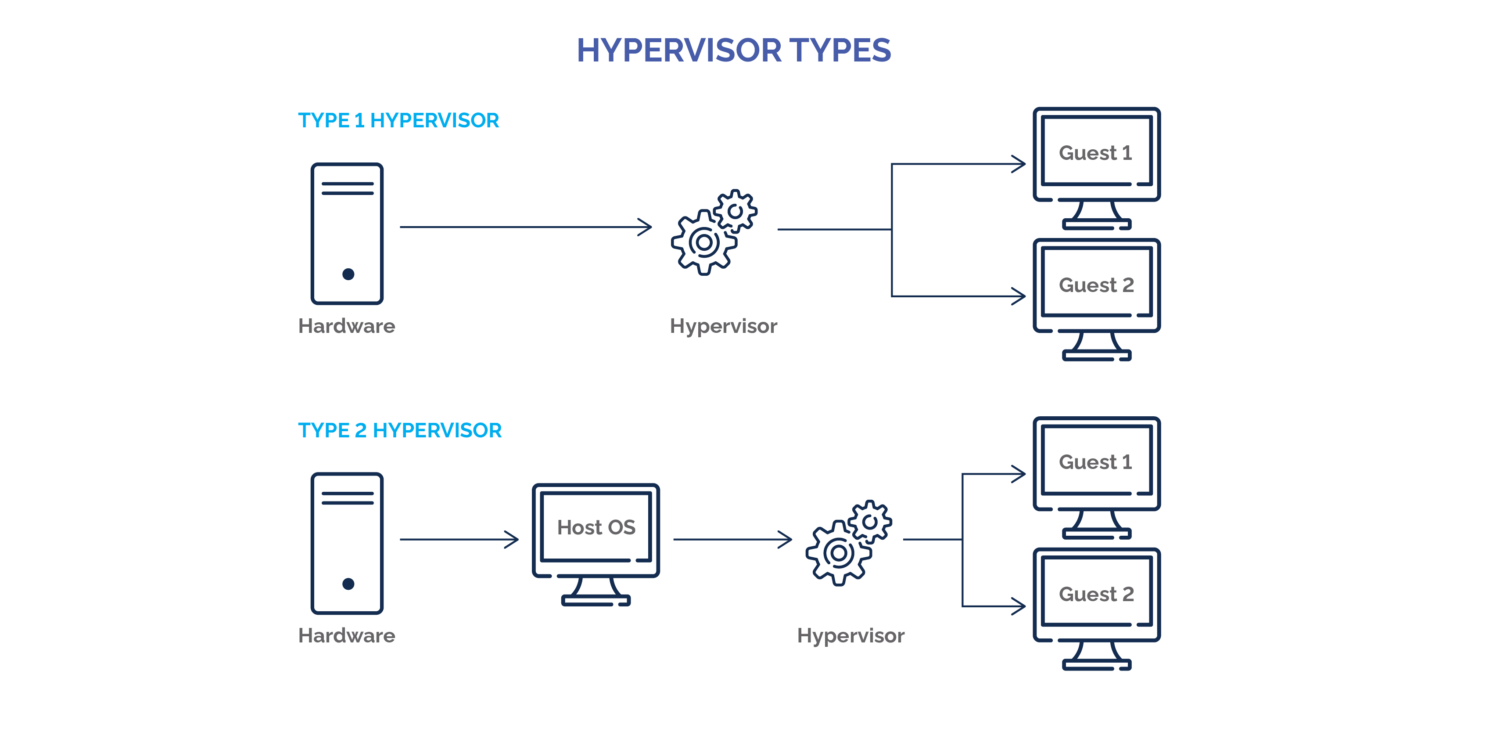
\includegraphics[width=1\textwidth]
	{assets/pics/type-1-hypervisor-vs-type-2.png}
	\caption{Hypervisor Type 1 vs Type 2}
	\label{fig:HypervisorType1vsType2}
\end{figure}

Pada Gambar \ref{fig:HypervisorType1vsType2} diperlihatkan diagram sederhana perbedaan daripada Hypervisor tipe 1 dan Hypervisor tipe 2. Hypervisor tipe 1 dan tipe 2 merupakan perangkat lunak yang digunakan untuk menjalankan satu atau lebih \vm\ (VM) pada satu mesin fisik. \vm\ adalah replika digital dari mesin fisik, menciptakan lingkungan komputasi terisolasi yang pengguna alami sebagai sepenuhnya independen dari perangkat keras yang mendasarinya\cite{hypervisor1vs2}. Hypervisor mengelola dan mengalokasikan sumber daya fisik ke VM dan berkomunikasi dengan perangkat keras di latar belakang. Hypervisor tipe 1 ditempatkan di atas server tanpa sistem operasi dan memiliki akses langsung ke sumber daya perangkat keras, sehingga dikenal juga sebagai \f{bare metal} hypervisor. Sebaliknya, hypervisor tipe 2 adalah aplikasi yang diinstal pada sistem operasi host dan juga dikenal sebagai \f{hosted} atau \f{embedded} hypervisor\cite{hypervisor1vs2}.


%-----------------------------------------------------------------------------%
\section{KVM \f{(Kernel-Based Virtual Machine)}}
%-----------------------------------------------------------------------------%

KVM (Kernel-based Virtual Machine) merupakan modul virtualisasi \oss\ dan gratis dalam kernel Linux yang memungkinkan kernel berfungsi sebagai hypervisor. KVM adalah hypervisor tipe 1 atau biasa juga disebut sebagai hypervisor \f{bare metal}. KVM memungkinkan mesin host menjalankan beberapa lingkungan virtual terisolasi yang disebut sebagai guest atau \vm\ (VM).KVM (Kernel-based Virtual Machine) merupakan modul virtualisasi sumber terbuka dan gratis dalam kernel Linux yang memungkinkan kernel berfungsi sebagai hypervisor. Ini adalah tipe-1 (bare-metal) hypervisor yang memungkinkan mesin host menjalankan beberapa lingkungan virtual terisolasi yang disebut sebagai guest atau mesin virtual (VM).

KVM telah disatukan ke dalam kernel Linux utama pada versi 2.6.20, yang dirilis pada 5 Februari 2007. Untuk dapat berjalan, KVM memerlukan prosesor dengan ekstensi virtualisasi perangkat keras, seperti Intel VT atau AMD-V. KVM menyediakan abstraksi perangkat tetapi tidak ada emulasi prosesor. Modul ini mengekspos antarmuka /dev/kvm, yang dapat digunakan oleh mode pengguna untuk menyiapkan ruang alamat VM guest.

KVM mendukung virtualisasi perangkat keras untuk berbagai sistem operasi guest, termasuk BSD, Solaris, Windows, Haiku, ReactOS, Plan 9, dan lainnya. Sebagai bagian dari kernel Linux, KVM langsung mengambil manfaat dari setiap fitur baru, perbaikan, dan kemajuan Linux tanpa perlu rekayasa tambahan.

Dalam pengaturan KVM, CPU virtual dari VM diimplementasikan sebagai thread (disebut "virtual CPU" atau vcpu) yang dijadwalkan oleh \f{Linux Kernel Scheduler}. KVM pada dasarnya adalah pengemudi untuk ekstensi virtualisasi processor. Setiap kali \f{Linux Scheduler} memilih tugas untuk dijalankan pada CPU fisik, dan tugas tersebut dikerjakan oleh CPU virtual dari VM, KVM "dihubungi" untuk memastikan bahwa yang sebenarnya berjalan di perangkat keras adalah program dari OS guest\cite{Abeni2020}.

\begin{figure}
	\centering
	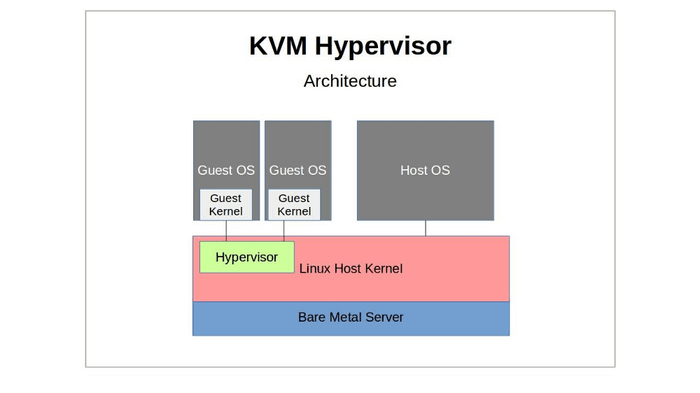
\includegraphics[width=1\textwidth]
	{assets/pics/xen-kvm.png}
	\caption{Arsitektur Hypervisor KVM}
	\label{fig:xen-kvm}
\end{figure}

Pada Gambar \ref{fig:xen-kvm} adalah struktur daripada hypervisor KVM. KVM berjalan langsung pada kernel linux host dan membagikan resourcenya kepada guest \vm, sedangkan sistem operasi host berjalan langsung diatas kernel host. Sistem operasi host dapat melakukan konfigurasi kepada \vm\ yang menggunakan hypervisor miliknya.

%-----------------------------------------------------------------------------%
\section{\f{Virtual Machine}}
%-----------------------------------------------------------------------------%

Virtual Machine (VM) adalah sebuah lingkungan komputasi yang dibuat secara virtual di dalam sebuah komputer fisik (host)\cite{Pradilla2016}. VM ini berfungsi seperti sebuah komputer independen yang dapat menjalankan sistem operasi dan aplikasi seperti komputer fisik biasa, tetapi semuanya berjalan dalam lingkungan virtual yang terisolasi di dalam host fisik. Setiap \vm\ (VM) menjalankan sistem operasi secara independen dan beroperasi terpisah dari VM lainnya, bahkan ketika semuanya berjalan pada host yang sama. Perangkat lunak yang dikenal sebagai hypervisor atau \vmm\ (VMM) memungkinkan kita untuk menjalankan berbagai sistem operasi yang berbeda secara bersamaan pada \vm\ yang berbeda. VM memiliki beberapa keunggulan dibandingkan dengan mesin fisik, termasuk kemampuan untuk menjalankan beberapa lingkungan sistem operasi pada satu komputer fisik, mendukung aplikasi \f{legacy}, dan menyediakan opsi pemulihan dalam situasi bencana. VM digunakan untuk berbagai keperluan, seperti \cc, pengujian sistem operasi baru, dan menjalankan beberapa aplikasi pada satu mesin fisik\cite{ibmWhatVirtualMachine}.

\begin{figure}
	\centering
	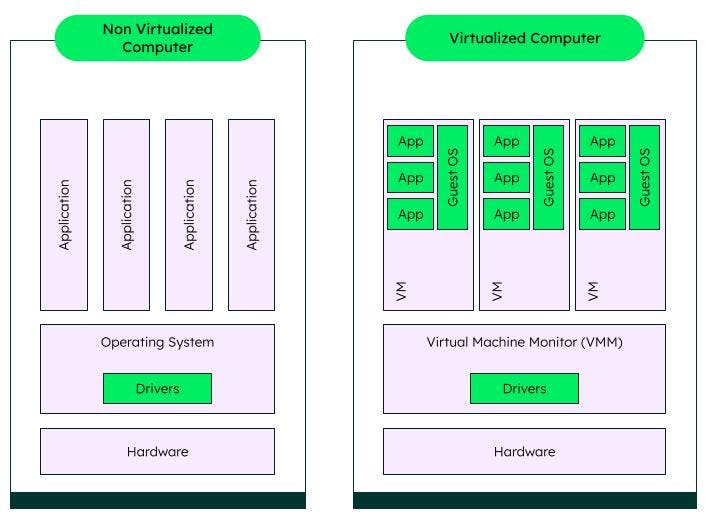
\includegraphics[width=1\textwidth]
	{assets/pics/vm-diagram.jpg}
	\caption{Perbedaan Komputasi Tanpa Virtualisasi dengan Virtualisasi}
	\label{fig:vm-diagram}
\end{figure}

Terdapat perbedaan dalam cara berjalan antara komputer tanpa virtualisasi (host) dan komputer yang divirtualisasi (guest) atau \vm. Pada Gambar 2.4, dapat diperlihatkan bahwa pada komputer tanpa virtualisasi, sistem operasinya berjalan langsung di atas perangkat keras, dengan driver yang berfungsi sebagai jembatan, sehingga aplikasi dapat berjalan langsung di atas sistem operasi tersebut. Di sisi lain, pada komputer yang divirtualisasi, sistem operasinya berjalan di atas VMM atau Virtual Machine Monitor, di mana satu VMM dapat menjalankan banyak sistem operasi guest.

%-----------------------------------------------------------------------------%
\section{\f{Advanced Encryption Standard} (AES)}
%-----------------------------------------------------------------------------%
\f{Advanced Encryption Standard} atau disingkat AES pertama kali diumumkan oleh NIST \f{(National Institute Of Standards and Technology)} pada tahun 2001 sebagai pengganti algoritma DES yang semakin mudah diretas. AES merupakan hasil dari kompetisi yang diadakan oleh NIST pada tahun 1997 yang dimenangkan oleh tim dari belgium yang memiliki nama asli Rijndael. Rijndael dikembangkan oleh dua orang kriptografer dari belgium bernama Joan Daemen dan Vincent Rijmen. AES dipublikasikan oleh NIST pada tahun 2001 dan tersebar secara efektif pada bulan May 2002 setelah disetujui oleh Menteri Perdagan Amerika, Donald Evans\cite{Kaffahemailencryptaes}.

AES merupakan metode enkripsi data dengan teknik enkripsi simetris, yang berarti menggunakan kunci yang sama untuk proses enkripsi dan dekripsi. Kunci pada AES tersedia dalam tiga varian ukuran, yakni 128 bit, 192 bit, dan 256 bit. Meskipun ukuran kuncinya bervariasi, ukuran blok data yang dienkripsi tetap sama, yaitu 128 bit. Ukuran blok mengacu pada cara data dienkripsi dengan memecah dan menyusunnya. Data disusun menjadi array 4x4 berukuran 16 byte, di mana setiap byte terdiri dari 8 bit, sehingga total setiap blok berjumlah 128 bit\cite{NistAes}.



%-----------------------------------------------------------------------------%
\section{\f{Cyclic Redundancy Check} (CRC)}
%-----------------------------------------------------------------------------%
\f{Cyclic Redundancy Check} (CRC) merupakan teknik yang digunakan untuk mendeteksi kesalahan dalam transmisi data digital. Teknik ini melibatkan penambahan kode pemeriksaan pada data untuk mengidentifikasi kesalahan yang mungkin terjadi selama proses transmisi. CRC didasarkan pada konsep pembagian polinomial, khususnya dengan menggunakan \f{Linear Feedback Shift Registers} (LFSRs).

\begin{enumerate}
	\item Gambaran Teknik CRC\cite{zhangLowComplexityCRC}:
	      \begin{itemize}
		      \item CRC digunakan untuk mendeteksi kesalahan dalam data digital, terutama pada aplikasi yang beroperasi dengan kecepatan tinggi.
		      \item CRC menggunakan \f{Linear Feedback Shift Registers} untuk deteksi kesalahan.
		      \item Teknik ini melibatkan pembagian biner untuk menghasilkan sisa (CRC) yang kemudian ditambahkan ke data sebagai pemeriksaan kesalahan di penerima.
	      \end{itemize}

	\item Prinsip CRC\cite{SrideviCRCDataRecovery}:
	      \begin{itemize}
		      \item Teknik CRC menambahkan kode pemeriksaan r-bit ke kode informasi k-bit, membentuk kode (n, k) dengan panjang n(k + r) bit.
		      \item Setiap kode (n, k) memiliki polinomial g(x) dengan kekuatan maksimum n-k=r terkait dengannya, dikenal sebagai polinomial yang dihasilkan dari kode CRC.
		      \item Kode CRC umumnya ditempatkan di akhir informasi untuk mendeteksi kesalahan selama transmisi.
		      \item Di sisi penerima, perhitungan CRC dilakukan pada informasi yang diterima untuk memeriksa kesalahan.
		      \item Implementasi seperti CRC-5, CRC-8, dan CRC-32 menunjukkan optimasi dan efisiensi yang spesifik untuk protokol dan sistem yang berbeda.
	      \end{itemize}
\end{enumerate}


%-----------------------------------------------------------------------------%
\section{virsh}
%-----------------------------------------------------------------------------%

virsh adalah \f{command line tool} yang merupakan bagian dari \f{library} libvirt dan secara utama digunakan untuk mengelola dan berinteraksi dengan teknologi virtualisasi pada sistem Linux, khususnya KVM (Kernel-based Virtual Machine) dan QEMU (Quick Emulator), dan mendukung hypervisor lainnya seperti Xen, LXC, OpenVZ, VirtualBox, dan VMware ESX\cite{libvirtLibvirtVirsh}.

Secara sederhana penggunaan virsh adalah seperti ini
\begin{center}
	\begin{verbatim}
		virsh [OPTION]... <command> <domain> [ARG]...
	\end{verbatim}
\end{center}

Pada command ini, domain adalah ID domain numerik, atau nama domain, atau UUID domain; dan ARGS adalah opsi khusus dari command. Setiap command yang dimulai dengan \# dianggap sebagai komentar dan diabaikan oleh sistem, semua perintah yang tidak dikenali akan didiagnosis.

%-----------------------------------------------------------------------------%
\section{\f{Streaming SIMD Extensions}}
%-----------------------------------------------------------------------------%
Streaming SIMD Extensions (SSE) adalah instruksi yang dibawa oleh Intel pada tahun 1999 dengan prosesor Pentium III dengan tujuan untuk meningkatkan kinerja prosesor arsitektur x86. Awalnya dikenal sebagai Katmai New Instructions (KNI) selama pengembangan, SSE secara signifikan meningkatkan kemampuan pemrosesan multimedia dan grafis dibanding pendahulunya, MMX. SSE mencakup 70 instruksi baru yang dirancang untuk meningkatkan tugas seperti pengolahan gambar, video 3D, audio dan video streaming, serta pengenalan suara\cite{informitStreamingSIMD}.

Tidak seperti pendahulunya, MMX menggunakan unit floating-point standar yang sama, sedangkan SSE menggunakan unit terpisah dalam prosesor untuk perhitungan floating-point, yang memungkinkan pemrosesan yang lebih efisien. SSE mendukung operasi floating-point SIMD (Single Instruction Multiple Data) single precision, yang sangat penting untuk mengatasi bottleneck dalam pemrosesan grafis 3D. Teknologi ini memungkinkan satu instruksi untuk melakukan hingga empat operasi floating-point secara bersamaan, meningkatkan kecepatan dan efisiensi pemrosesan\cite{informitStreamingSIMD}.

Manfaat SSE yang utama terlihat dalam decoding MPEG2, format standar untuk video DVD, memungkinkan prosesor yang dilengkapi SSE untuk menangani decoding tersebut di perangkat lunak dengan kecepatan penuh tanpa perangkat keras tambahan. SSE juga meningkatkan penggunaan CPU dan kinerja perangkat lunak pengenalan suara, memberikan akurasi yang lebih tinggi dan waktu respons yang lebih cepat. Untuk sepenuhnya memanfaatkan kemampuan SSE, aplikasi harus diset secara khusus agar SSE-aware, sebuah fitur yang sekarang umum dalam banyak aplikasi grafis dan berhubungan dengan suara. SSE adalah perluasan dari MMX, yang berarti bahwa prosesor yang mendukung SSE juga kompatibel dengan instruksi MMX, hal ini memastikan \f{backward compatibility} dengan aplikasi yang mendukung MMX\cite{informitStreamingSIMD}.

SSE telah berkembang seiring waktu dengan versi seperti SSE2, SSE3, dan SSE4, masing-masing membawa fitur baru dan meningkatkan kemampuan pemrosesan secara keseluruhan. Ekstensi ini telah banyak diadopsi dalam pengembangan perangkat lunak, terutama dalam bidang di mana pemrosesan paralel sangat penting.

\subsection{SSE2}
SSE2 adalah perluasan dari kemampuan SIMD (Single Instruction, Multiple Data) yang awalnya diperkenalkan dengan set instruksi SSE (Streaming SIMD Extensions). Pertama kali diperkenalkan oleh Intel dengan prosesor Pentium 4\cite{SystemVAppBinaryInterfaceMichael}. Perbedaan utama dan peningkatan dalam SSE2 dibandingkan dengan pendahulunya SSE meliputi:

\begin{enumerate}
	\item Rentang Jenis Data yang Lebih Luas

	      SSE2 memperluas kemampuan SIMD untuk beroperasi pada data integer 64-bit dan data floating-point presisi ganda (SSE terutama berfokus pada operasi floating-point presisi tunggal).

	\item Peningkatan Set Instruksi

	      SSE2 menambahkan instruksi dan kemampuan baru, meningkatkan pengolahan dan manipulasi berbagai jenis data, termasuk integer terpak (packed integers) dan angka floating-point presisi ganda.

	\item Peningkatan Kinerja untuk Aplikasi Ilmiah dan Multimedia

	      Dengan menyediakan operasi pada tipe data yang lebih besar dan set operasi yang lebih luas, SSE2 meningkatkan efisiensi dan kinerja aplikasi yang berhubungan dengan perhitungan matematika kompleks, grafik 3D, pengkodean video, dan tugas multimedia lainnya.
\end{enumerate}

Penggabungan SSE2 dalam arsitektur AMD64 menyoroti pentingnya dalam komputasi modern, terutama untuk aplikasi yang memerlukan kinerja tinggi dalam pengolahan numerik dan multimedia. Dokumen ABI kemungkinan mengasumsikan keakraban dengan konsep-konsep ini, lebih berfokus pada detail implementasi dalam arsitektur AMD64 daripada menjelaskan perbedaan fundamental antara SSE dan SSE2\cite{SystemVAppBinaryInterfaceMichael}.

\subsection{SSE3}
SSE3 (Streaming SIMD Extensions 3) merupakan ekstensi dari set instruksi SSE2, yang mana memperluas teknologi SSE (Streaming SIMD Extensions) asli. Perbedaan antara SSE3 dengan SSE2 antara lain:

\begin{enumerate}
	\item 13 Set Instruksi Baru

	      SSE3 menambahkan tiga belas instruksi baru ke set instruksi SSE/SSE2 yang ada\cite{Hassaballah2008}.

	\item Dukungan untuk Model Eksekusi SIMD:

	      Dari 13 instruksi ini, sepuluh dirancang untuk mendukung model eksekusi SIMD (Single Instruction, Multiple Data). Model ini merupakan aspek penting dari komputasi paralel, di mana beberapa titik data diproses secara bersamaan menggunakan satu instruksi. Ini sangat bermanfaat untuk tugas-tugas seperti pengolahan grafis, perhitungan ilmiah, dan aplikasi multimedia, di mana operasi pada set data besar adalah hal yang umum\cite{Hassaballah2008}.

	\item Konversi Floating-Point ke Integer:

	      Salah satu instruksi SSE3 secara spesifik mempercepat pemrograman \f{x87-style}. Instruksi ini berfokus pada peningkatan efisiensi dalam mengkonversi nilai floating-point menjadi integer. Hal ini bisa sangat berguna dalam skenario di mana perhitungan melibatkan tipe data floating-point dan integer\cite{Hassaballah2008}.

	\item Akselerasi Sinkronisasi Thread:

	      Dua instruksi lain dalam set SSE3 ditujukan untuk meningkatkan sinkronisasi thread. Peningkatan ini sangat penting dalam aplikasi multi-thread, di mana pengelolaan eksekusi dan koordinasi beberapa thread adalah kunci untuk kinerja yang baik dan efisiensi\cite{Hassaballah2008}.
\end{enumerate}

Secara singkat, SSE3 memperluas kemampuan set instruksi SSE dan SSE2 dengan penekanan pada peningkatan eksekusi SIMD, konversi floating-point ke integer, serta sinkronisasi thread. Selain itu, SSE3 tetap mempertahankan kompatibilitas dengan jenis data dan lingkungan pemrograman yang sudah ada. Oleh karena itu, SSE3 menjadi alat yang sangat berguna bagi pengembang yang bekerja pada tugas komputasi berkinerja tinggi, terutama yang melibatkan pemrosesan paralel dan jenis data yang kompleks.

\subsection{SSSE3}
SSSE3 (Supplemental Streaming SIMD Extensions 3) adalah ekstensi dari set instruksi SSE3 yang diperkenalkan oleh Intel pada tahun 2006. SSSE3 menambahkan 32 instruksi baru ke set instruksi SSE3 yang ada, yang dirancang untuk meningkatkan kinerja pemrosesan SIMD (Single Instruction, Multiple Data) pada aplikasi yang memerlukan operasi vektorisasi dan paralel. Pembaruan dari SSSE3 antara lain:

\begin{enumerate}
	\item Dua belas instruksi yang melakukan operasi penambahan atau pengurangan horizontal.
	\item Enam instruksi yang mengevaluasi nilai absolut.
	\item Dua instruksi yang melakukan operasi perkalian-dan-penambahan dan mempercepat evaluasi \f{dot product}.
	\item Dua instruksi yang mempercepat operasi perkalian bilangan bulat dan menghasilkan nilai bilangan bulat dengan penskalaan.
	\item Dua instruksi yang melakukan \f{in-place shuffle} pada tingkat byte sesuai dengan operand kontrol pengacakan kedua.
	\item Enam instruksi yang mengubah bilangan bulat menjadi negatif dalam operand tujuan jika elemen yang sesuai dalam operand sumber adalah negatif.
	\item Dua instruksi yang menyelaraskan data dari gabungan dua operand.
\end{enumerate}

\subsection{SSE4}
SSE4, yang merupakan singkatan dari Streaming SIMD Extensions 4, adalah serangkaian instruksi yang diperkenalkan oleh Intel dalam prosesor 64-bitnya yang dibuat dengan teknologi proses 45 nm. SSE4 terdiri dari dua subset: SSE4.1 dan SSE4.2\cite{sse4reference}.

\begin{table}[h]
	\centering
	\begin{tabular}{|p{3cm}|p{4.6cm}|p{4.6cm}|}
		\hline
		\textbf{Fitur}      & \textbf{SSE4.1}                                                               & \textbf{SSE4.2}                                                     \\ \hline
		Pengenalan          & Bagian dari prosesor Intel 45 nm                                              & Diperkenalkan dengan arsitektur mikro Nehalem                       \\ \hline
		Instruksi           & 47 set instruksi baru                                                         & 7 instruksi tambahan                                                \\ \hline
		Fokus               & Peningkatan kinerja pada media, pengolahan citra, dan beban kerja 3D          & Pengolahan string dan teks                                          \\ \hline
		Penyempurnaan Utama & Peningkatan vektorisasi kompiler, dukungan untuk perhitungan \f{packed dword} & Kemampuan integer SIMD yang ditingkatkan, fokus pada operasi string \\ \hline
		Kompatibilitas      & Sepenuhnya kompatibel dengan versi SSE sebelumnya                             & Juga kompatibel dengan versi SSE sebelumnya                         \\ \hline
		Dukungan OS         & Tidak memerlukan dukungan OS baru                                             & Sama seperti SSE4.1                                                 \\ \hline
	\end{tabular}
	\caption{Perbandingan SSE4.1 dan SSE4.2}
	\label{table:perbandingan_sse4}
\end{table}

Berdasarkan informasi dalam tabel \ref{table:perbandingan_sse4}, SSE4.1 dirancang untuk meningkatkan performa dalam aplikasi media, pencitraan, dan 3D, serta menghadirkan 47 instruksi baru. Instruksi-instruksi ini berkontribusi pada peningkatan vektorisasi kompiler dan memberikan dukungan untuk perhitungan \f{packed dword}. Di sisi lain, SSE4.2, yang pertama kali diperkenalkan dalam prosesor dengan mikroarsitektur Nehalem, menambahkan tujuh instruksi tambahan. Fokus utama dari instruksi-instruksi tambahan ini adalah pada pemrosesan string dan teks, serta peningkatan dalam kemampuan integer SIMD\cite{sse4reference}.

SSE4 tidak memperkenalkan tipe data baru tetapi mencakup berbagai tipe instruksi seperti perkalian dword, \f{floating-point dot-product}, \f{streaming load hint}, \f{packed blending}, dan instruksi MIN/MAX \f{packed integer}. Teknologi ini bertujuan untuk meningkatkan dukungan untuk perhitungan \f{packed dword} dan meningkatkan throughput memori untuk jenis memori tertentu. SSE4 sepenuhnya kompatibel dengan perangkat lunak dari generasi sebelumnya dari prosesor Intel dan tidak memerlukan dukungan OS baru di luar apa yang diperlukan untuk Streaming SIMD Extensions (SSE) sebelumnya\cite{sse4reference}.
%-----------------------------------------------------------------------------%
\chapter{\babTiga}
%-----------------------------------------------------------------------------%
Penelitian ini bertujuan untuk mengevaluasi konfigurasi Hypervisor KVM yang disediakan secara langsung dalam konteks penggunaan \vm\ pada Apache Cloudstack. Tujuan utama adalah untuk memastikan bahwa \vm\ dapat mencapai kinerja yang optimal sesuai dengan spesifikasi sistem yang digunakan. Untuk mencapai tujuan ini, \saya\ akan melakukan penyesuaian konfigurasi atau tuning pada Hypervisor KVM dan kemudian membandingkannya dengan kondisi awal yang tidak mengalami tuning. Hasil pengujian akan dianalisis untuk menentukan apakah ada perbedaan signifikan dalam kinerja antara Hypervisor KVM yang telah dituning dengan yang belum dituning.

%-----------------------------------------------------------------------------%
\section{Tahapan Penelitian}
%-----------------------------------------------------------------------------%
\begin{figure}
    \centering
    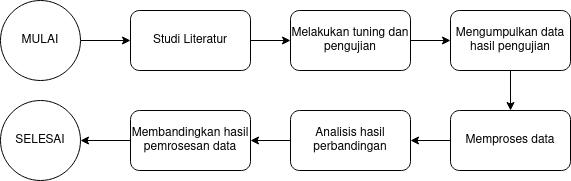
\includegraphics[width=1\textwidth]
    {assets/pics/tahapan-penelitian.png}
    \caption{Tahapan Penelitian}
    \label{fig:TahapanPenelitian}
\end{figure}

Penelitian ini akan dilakukan dalam beberapa tahap sesuai dengan diagram di gambar \ref{fig:TahapanPenelitian}. Tahap pertama melibatkan studi literatur untuk mengumpulkan semua informasi yang diperlukan. Studi literatur ini penting karena memberikan dasar pengetahuan yang kuat tentang topik yang akan diteliti, memungkinkan peneliti untuk memahami konteks dan kerangka kerja yang relevan.

Selanjutnya, penelitian melibatkan tuning terhadap Hypervisor KVM, dan pengujian dilakukan dengan tiga skenario, yaitu kompresi video, enkripsi data dengan AES, dan validasi integritas data menggunakan CRC32. Hasil dari pengujian ini akan memberikan gambaran mengenai konfigurasi yang paling optimal dan sesuai, serta membantu dalam pemahaman lebih lanjut tentang pengaruh tuning terhadap performa Hypervisor KVM.

%-----------------------------------------------------------------------------%
\section{Persiapan Lingkungan untuk Pengujian dan Analisis}
%-----------------------------------------------------------------------------%
\begin{figure}
    \centering
    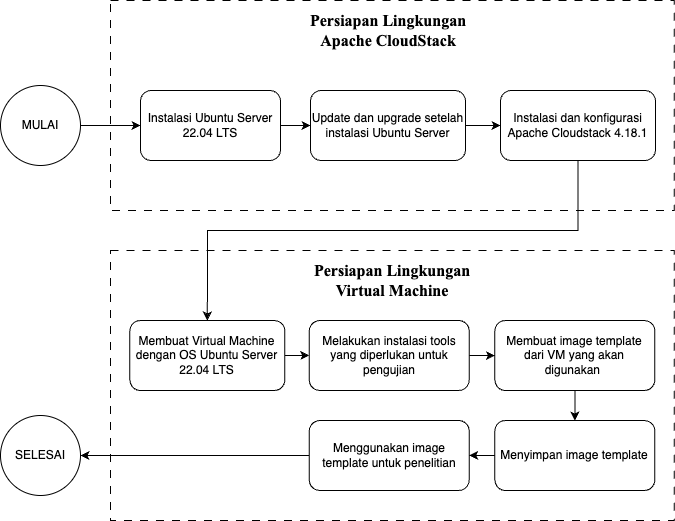
\includegraphics[width=1\textwidth]
    {assets/pics/persiapan_lingkungan_penelitian.png}
    \caption{Persiapan Lingkungan Penelitian}
    \label{fig:PersiapanLingkunganPenelitian}
\end{figure}


Proses persiapan lingkungan untuk pengujian dan analisis yang tergambar dalam gambar \ref{fig:PersiapanLingkunganPenelitian} menggambarkan serangkaian langkah sistematis yang penting untuk memastikan integritas hasil penelitian. Proses ini dimulai dengan tahap inisiasi yang meliputi instalasi Ubuntu Server 22.04 LTS, sebuah sistem operasi yang stabil dan sering digunakan untuk keperluan server. Instalasi ini menjadi landasan dasar bagi infrastruktur yang akan dikembangkan.

Setelah sistem operasi terinstal, dilakukan pembaruan dan peningkatan sistem operasi tersebut untuk memastikan semua komponen sistem berada pada versi terkini serta keamanan sistem terjaga. Langkah ini krusial untuk menutup potensi kerentanan yang mungkin ada pada sistem. Selanjutnya, Apache Cloudstack versi 4.18.1 diinstal dan dikonfigurasikan. Apache Cloudstack berfungsi sebagai platform manajemen cloud yang memungkinkan pembuatan dan pengelolaan infrastruktur cloud yang kompleks, yang merupakan elemen kunci dalam penelitian ini.

Dalam pembuatan lingkungan virtual, dibuat \vm\ yang menggunakan sistem operasi yang sama, yaitu Ubuntu Server 22.04 LTS. Pembuatan VM ini memungkinkan simulasi berbagai skenario penelitian dalam lingkungan yang terisolasi. Selanjutnya, untuk keperluan analisis dan pengujian, berbagai perangkat lunak yang akan digunakan untuk melakukan pengujian akan di install.

Tahapan selanjutnya merupakan pembuatan image template dari VM yang telah dikonfigurasikan. Proses ini memungkinkan duplikasi VM dengan cepat dan efisien untuk pengujian berulang atau skenario analisis yang berbeda, menjamin konsistensi lingkungan penelitian. Image template ini kemudian digunakan sebagai standar untuk penelitian lebih lanjut, memastikan bahwa setiap VM yang dibuat untuk tujuan pengujian memiliki konfigurasi yang identik.

Setelah semua dilakukan hal ini menandakan bahwa lingkungan penelitian telah siap untuk diuji dan dianalisis. Kesiapan lingkungan ini esensial untuk memastikan bahwa pengujian yang dilakukan dapat diulang dengan cepat dan efisien.

%-----------------------------------------------------------------------------%
\subsection{Instalasi dan Konfigurasi Apache Cloudstack}
%-----------------------------------------------------------------------------%
Dalam instalasi ini akan digunakan \f{Home Network} di IP 192.168.0.0/24. Pertama pastikan bahwa \f{tools} yang dibutuhkan sudah terinstall dengan perintah:

\begin{lstlisting}
    sudo apt-get install -y openntpd openssh-server vim htop tar
    sudo apt-get install -y intel-microcode
\end{lstlisting}

Perintah ini akan menginstall \f{tools} openntpd, openssh-server, vim, htop, tar, dan intel-microcode. Setelah melakukan instalasi \f{tools} ini kemudian \saya\ akan mengganti password dari user root dengan perintah:

\begin{lstlisting}
    sudo passwd root
\end{lstlisting}

%-----------------------------------------------------------------------------%
\subsubsection{Pengaturan Jaringan}
%-----------------------------------------------------------------------------%
Melakukan pengaturan \f{Linux Bridge} yang akan menghandle jaringan CloudStack \f{public, guest, management} dan \f{storage}. Untuk penyederhanaan \saya\ akan menggunakan satu \f{bridge} yang bernama \textbf{cloudbr0} yang akan digunakan untuk semua jaringan ini. Untuk menginstall \f{tools} untuk melakukan \f{bridge} digunakan perintah:

\begin{lstlisting}
    sudo apt-get install bridge-utils
\end{lstlisting}

Setelah menginstall \f{tools} ini, \saya\ akan mengkonfigurasi \f{bridge} cloudbr0 dengan menggunakan netplan. Pertama pastikan bahwa seleuruh konfigurasi netplan sekarang di rename dengan menambahkan extensi .bak sebagai backup. Setelah itu buat file konfigruasi netplan dengan perintah:

\begin{lstlisting}
    sudo nano /etc/netplan/01-netcfg.yaml
\end{lstlisting}

Dengan perintah ini akan membuka text editor nano dengan file 01-netcfg.yaml. Isi file konfigurasi tersebut dengan:

\begin{listing}[H]
    \begin{minted}{yaml}
    network:
        version: 2
        renderer: networkd
        ethernets:
            enp2s0:
                dhcp4: false
                dhcp6: false
                optional: true
        bridges:
            cloudbr0:
                addresses: [192.168.0.10/24]
                routes:
                -   to: default
                    via: 192.168.0.1
                nameservers:
                    addresses: [1.1.1.1,8.8.8.8]
                interfaces: [enp2s0]
                dhcp4: false
                dhcp6: false
                parameters:
                    stp: false
                    forward-delay: 0
    \end{minted}
    \caption{Konfigurasi Netplan untuk Cloudbr0}
    \label{code:netplan_config}
\end{listing}

Dalam konfigurasi ini IP dari \f{bridge} cloudbr0 adalah 192.168.0.10/24 dan akan menggunakan DNS 1.1.1.1 dan 8.8.8.8. Setelah melakukan konfigurasi ini \saya\ akan mengaktifkan \f{bridge} cloudbr0 dengan perintah:

\begin{lstlisting}
    sudo netplan generate
    sudo netplan apply
    sudo reboot
\end{lstlisting}

Dengan perintah ini akan dilakukan netplan generate dan apply, setelah itu sistem melakukan reboot. Sampai sini pembuatan \f{bridge} cloudbr0 sudah selesai.

\subsubsection{Instalasi Cloudstack}
Pertama kita akan melakukan instalasi cloudstack-management dan juga mysql-server. Database yang akan digunakan adalah MySQL. Kita akan menggunakan perintah:

\begin{lstlisting}
    sudo mkdir -p /etc/apt/keyrings
    wget -O- http://packages.shapeblue.com/release.asc | gpg --dearmor | sudo tee /etc/apt/keyrings/cloudstack.gpg > /dev/null
    
    echo deb [signed-by=/etc/apt/keyrings/cloudstack.gpg] http://packages.shapeblue.com/cloudstack/upstream/debian/4.18 / > /etc/apt/sources.list.d/cloudstack.list \\
    sudo apt-get update -y
    sudo apt-get install cloudstack-management mysql-server
\end{lstlisting}

Perintah tersebut digunakan untuk menginstal CloudStack Management Server versi 4.18 dan MySQL Server dari repositori tertentu. Pertama, perintah membuat direktori untuk menyimpan kunci GPG yang digunakan untuk mengotentikasi paket dari repositori CloudStack. Kemudian, kunci GPG tersebut diunduh, didekompresi, dan disimpan dalam direktori yang telah dibuat. Selanjutnya, konfigurasi ditambahkan ke file sources.list.d untuk menandatangani paket-paket dari repositori CloudStack. Setelah itu, daftar paket diperbarui dan CloudStack Management Server serta MySQL Server diinstal menggunakan perintah apt-get. Selain ini juga akan dilakukan instalasi \f{tools} cloudstack usage dan billing yang bersifat opsional, dengan perintah:

\begin{lstlisting}
    sudo apt-get install cloudstack-usage
\end{lstlisting}

\subsubsection{Konfigurasi Database}
Setelah mysql server selesai di install akan dilakukan konfigurasi setting InnoDB di mysql server dengan perintah:

\begin{lstlisting}
    sudo nano /etc/mysql/mysql.conf.d/mysqld.cnf
\end{lstlisting}

Hapus semua isi file tersebut dan isi dengan:

\begin{listing}[H]
    \begin{minted}{ini}
    [mysqld]

    server_id = 1
    sql-mode="STRICT_TRANS_TABLES,NO_ENGINE_SUBSTITUTION,ERROR_FOR_DIVISION_BY_ZERO
    NO_ZERO_DATE,NO_ZERO_IN_DATE,NO_ENGINE_SUBSTITUTION"
    innodb_rollback_on_timeout=1
    innodb_lock_wait_timeout=600
    max_connections=1000
    log-bin=mysql-bin
    binlog-format = 'ROW'
    \end{minted}
    \caption{Konfigurasi mysqld.cnf}
    \label{code:mysql_config}
\end{listing}

Simpan konfigurasi dan setelah itu restart mysql server. Hal ini dilakukan agar mysql menggunakan setting yang terbaru. Untuk melakukan restart mysql server dapat dilakukan dengan perintah:

\begin{lstlisting}
    systemctl restart mysql
\end{lstlisting}

Setelah mysql server selesai di restart langkah selanjunya adalah deploy database untuk cloudstack. Deploy server ini harus dilakukan sebagai user root. Deploy dilakukan dengan perintah:

\begin{lstlisting}
    cloudstack-setup-databases cloud:cloud@localhost --deploy-as=root:password -i 192.168.0.10
\end{lstlisting}

IP yang digunakan adalah IP dari sistem host. Tunggu sampai deployment selesai, langkah ini akan selesai dalam beberapa menit.

\subsubsection{Konfigurasi Storage}
Pada tahap ini \saya\ akan melakukan konfigurasi untuk penyimpanan dari cloudstack. Pertama kita akan melakukan instalasi storage driver yang akan digunakan dengan perintah:

\begin{lstlisting}
    sudo apt-get install nfs-kernel-server quota
    echo "/export  *(rw,async,no_root_squash,no_subtree_check)" > /etc/exports
    sudo mkdir -p /export/primary /export/secondary
    sudo exportfs -a
\end{lstlisting}

Perintah \texttt{sudo apt-get install nfs-kernel-server quota} digunakan untuk menginstal perangkat lunak server NFS dan modul Quota pada sistem Linux. Selanjutnya, perintah \texttt{echo "/export *(rw,async,no\_root\_squash,no\_subtree\_check)" > /etc/exports} digunakan untuk menetapkan konfigurasi eksport NFS dengan opsi akses tertentu. Kemudian, perintah \texttt{sudo mkdir -p /export/primary /export/secondary} membuat direktori yang akan diakses oleh klien NFS. Terakhir, perintah \texttt{sudo exportfs -a} mengekspor semua direktori yang telah dikonfigurasi sebelumnya untuk diakses oleh klien NFS. Dengan demikian, rangkaian perintah ini mempersiapkan server NFS untuk berbagi data melalui jaringan. Setelah itu akan dilakukan konfigurasi NFS server dengan perintah:

\begin{lstlisting}
    sed -i -e 's/^RPCMOUNTDOPTS="--manage-gids"$/RPCMOUNTDOPTS="-p 892 --manage-gids"/g' /etc/default/nfs-kernel-server
    sed -i -e 's/^STATDOPTS=$/STATDOPTS="--port 662 --outgoing-port 2020"/g' /etc/default/nfs-common
    echo "NEED_STATD=yes" >> /etc/default/nfs-common
    sed -i -e 's/^RPCRQUOTADOPTS=$/RPCRQUOTADOPTS="-p 875"/g' /etc/default/quota
    service nfs-kernel-server restart
\end{lstlisting}

Perintah-perintah tersebut digunakan untuk mengubah konfigurasi pada server NFS dan Quota pada sistem Linux. Pertama, menggunakan \texttt{sed}, konfigurasi NFS Mount Daemon dan NFS Stat Daemon diubah untuk menggunakan port yang ditentukan dan mengaktifkan manajemen GID. Selanjutnya, layanan Stat Daemon diaktifkan dengan menambahkan opsi yang sesuai ke file konfigurasi NFS Common. Kemudian, konfigurasi RPC Quota Daemon diubah untuk menggunakan port yang ditentukan. Terakhir, layanan NFS Kernel Server di-restart untuk menerapkan perubahan konfigurasi yang telah dilakukan.

\subsubsection{Konfigurasi KVM}
Tahap selanjutnya adalah konfigurasi KVM dan cloudstack agent. Pertama install kvm dan cloudstack agent dengan perintah:

\begin{lstlisting}
    sudo apt-get install qemu-kvm cloudstack-agent
\end{lstlisting}

Setelah KVM dan cloudstack agent terinstall langkah selanjutnya adalah menjalankan perintah ini:

\begin{lstlisting}
    sudo sed -i -e 's/\#vnc_listen.*$/vnc_listen = "0.0.0.0"/g' /etc/libvirt/qemu.conf
    sudo echo LIBVIRTD_ARGS=\"--listen\" >> /etc/default/libvirtd
    sudo systemctl mask libvirtd.socket libvirtd-ro.socket libvirtd-admin.socket libvirtd-tls.socket libvirtd-tcp.socket
    sudo systemctl restart libvirtd
\end{lstlisting}

Perintah tersebut digunakan untuk mengkonfigurasi libvirt, sebuah toolkit untuk mengelola virtualisasi di Linux. Pertama, perintah \texttt{sed} digunakan untuk mengubah pengaturan dalam file konfigurasi \texttt{qemu.conf} agar libvirt dapat menerima koneksi VNC dari semua interface jaringan. Kemudian, argumen \texttt{--listen} ditambahkan ke konfigurasi libvirtd melalui file \texttt{/etc/default/libvirtd}, yang membuat libvirt mendengarkan koneksi dari interface jaringan. Selanjutnya, perintah \texttt{systemctl mask} digunakan untuk menonaktifkan unit-unit systemd yang terkait dengan libvirtd, seperti socket-soket yang tidak diperlukan, untuk menghindari aktivasi yang tidak diinginkan. Terakhir, layanan libvirtd di-restart agar perubahan konfigurasi dapat diterapkan.

Selanjutnya akan dilakukan konfigurasi default untuk libvirtd dengan perintah:

\begin{lstlisting}
    echo 'listen_tls=0' >> /etc/libvirt/libvirtd.conf
    echo 'listen_tcp=1' >> /etc/libvirt/libvirtd.conf
    echo 'tcp_port = "16509"' >> /etc/libvirt/libvirtd.conf
    echo 'mdns_adv = 0' >> /etc/libvirt/libvirtd.conf
    echo 'auth_tcp = "none"' >> /etc/libvirt/libvirtd.conf
    systemctl restart libvirtd
\end{lstlisting}

Perintah-perintah tersebut digunakan untuk mengkonfigurasi default pada file konfigurasi libvirt (libvirtd.conf). Pertama, dengan menambahkan \texttt{listen\_tls=0}, libvirt diminta untuk tidak mendengarkan koneksi TLS, sehingga mematikan mode tersebut. Kemudian, \texttt{listen\_tcp=1} mengaktifkan libvirt untuk mendengarkan koneksi TCP/IP. Penambahan \texttt{tcp\_port = "16509"} menetapkan port TCP yang akan digunakan oleh libvirt. Selanjutnya, dengan \texttt{mdns\_adv = 0}, mDNS advertise untuk penemuan otomatis layanan libvirt dimatikan. Terakhir, \texttt{auth\_tcp = "none"} mengatur libvirt untuk menerima koneksi TCP/IP tanpa melakukan otentikasi. Setelah perubahan-perubahan ini diterapkan, layanan libvirt di-restart agar konfigurasi baru dapat mulai berlaku. Penting untuk dicatat bahwa konfigurasi default ini hanya diperlukan saat setup awal, karena saat menambahkan host KVM dalam CloudStack, konfigurasi yang lebih aman menggunakan TLS akan diterapkan secara otomatis.

Pada host tertentu ditempat menjalankan docker dan service lainnya, dimungkinkan perlu untuk menambahkan konfigrasi berikut ini di \texttt{/etc/sysctl.conf} lalu jalankan \texttt{sysctl -p}

\begin{lstlisting}
    nano /etc/sysctl.conf
    echo 'net.bridge.bridge-nf-call-arptables = 0' >> /etc/sysctl.conf
    echo 'net.bridge.bridge-nf-call-iptables = 0' >> /etc/sysctl.conf
    sysctl -p
\end{lstlisting}

Pad perintah ini pertama, akan dibuka file \texttt{/etc/sysctl.conf} menggunakan editor teks nano. Kemudian, dengan menambahkan baris \texttt{net.bridge.bridge-nf-call-arptables = 0} dan \texttt{net.bridge.bridge-nf-call-iptables = 0} ke dalam file tersebut, Ini akan mematikan fungsi kernel yang biasanya dipanggil saat menggunakan Docker dan jembatan jaringan (bridge). Ini penting karena beberapa layanan, seperti Docker, kadang memerlukan konfigurasi khusus agar berjalan dengan lancar di lingkungan host yang kompleks. Terakhir, dengan menjalankan perintah \texttt{sysctl -p}, perubahan konfigurasi yang telah dibuat akan diterapkan tanpa harus me-reboot sistem, sehingga memungkinkan kernel untuk memuat ulang konfigurasi yang baru diterapkan.

Setelah itu kita akan mengenerate host id dengan uuid, hal ini dapat dilakukan dengan perintah:

\begin{lstlisting}
    sudo apt-get install uuid
    UUID=$(uuid)
    echo host_uuid = \"$UUID\" >> /etc/libvirt/libvirtd.conf
    systemctl restart libvirtd
\end{lstlisting}

Perintah ini digunakan untuk meng-generate UUID (Universally Unique Identifier) untuk host dan mengintegrasikannya ke dalam konfigurasi libvirtd. Perintah \texttt{UUID=\$(uuid)} digunakan untuk meng-generate UUID secara acak dan menyimpannya dalam variabel \texttt{UUID}. UUID adalah string panjang yang unik secara global dan digunakan untuk mengidentifikasi entitas secara unik di sistem. Kemudian, perintah \texttt{echo host\_uuid = \" \$UUID \"  >> /etc/libvirt/libvirtd.conf} menambahkan baris \texttt{host\_uuid = "<nilai UUID>"} ke dalam file konfigurasi \texttt{libvirtd.conf}. Fungsi baris ini adalah untuk menyimpan UUID host di konfigurasi libvirtd, yang akan digunakan oleh libvirt untuk mengidentifikasi host secara unik dalam lingkungan virtualisasi. Terakhir, perintah systemctl restart libvirtd digunakan untuk merestart layanan libvirtd agar perubahan konfigurasi yang telah dilakukan dapat diterapkan.

\subsubsection{Konfigurasi Firewall}
Untuk melakukan konfigruasi firewall kita dapat menggunakan perintah:

\begin{lstlisting}
    # configure firewall rules to allow useful ports
    NETWORK=192.168.0.0/24
    iptables -A INPUT -s $NETWORK -m state --state NEW -p udp --dport 111 -j ACCEPT
    iptables -A INPUT -s $NETWORK -m state --state NEW -p tcp --dport 111 -j ACCEPT
    iptables -A INPUT -s $NETWORK -m state --state NEW -p tcp --dport 2049 -j ACCEPT
    iptables -A INPUT -s $NETWORK -m state --state NEW -p tcp --dport 32803 -j ACCEPT
    iptables -A INPUT -s $NETWORK -m state --state NEW -p udp --dport 32769 -j ACCEPT
    iptables -A INPUT -s $NETWORK -m state --state NEW -p tcp --dport 892 -j ACCEPT
    iptables -A INPUT -s $NETWORK -m state --state NEW -p tcp --dport 875 -j ACCEPT
    iptables -A INPUT -s $NETWORK -m state --state NEW -p tcp --dport 662 -j ACCEPT
    iptables -A INPUT -s $NETWORK -m state --state NEW -p tcp --dport 8250 -j ACCEPT
    iptables -A INPUT -s $NETWORK -m state --state NEW -p tcp --dport 8080 -j ACCEPT
    iptables -A INPUT -s $NETWORK -m state --state NEW -p tcp --dport 9090 -j ACCEPT
    iptables -A INPUT -s $NETWORK -m state --state NEW -p tcp --dport 16514 -j ACCEPT
    
    apt-get install iptables-persistent
\end{lstlisting}

Perintah tersebut bertujuan untuk mengonfigurasi aturan firewall pada sistem menggunakan iptables, dengan fokus pada pembukaan port-port yang umum digunakan untuk layanan-layanan tertentu. Pertama, baris \texttt{NETWORK=192.168.0.0/24} mendefinisikan jaringan yang diizinkan melalui aturan firewall. Selanjutnya, setiap perintah \texttt{iptables -A INPUT ... -j ACCEPT} menambahkan aturan iptables untuk mengizinkan koneksi baru pada port tertentu dari jaringan yang telah ditentukan sebelumnya. Misalnya, perintah \texttt{iptables -A INPUT -s \$NETWORK -m state --state NEW -p udp --dport 111 -j ACCEPT} mengizinkan koneksi UDP baru pada port 111 dari jaringan yang telah ditentukan.

Aturan-aturan tersebut dirancang untuk membuka akses ke port-port yang umum digunakan oleh layanan-layanan seperti NFS, RPC, dan layanan manajemen tertentu. Setelah semua aturan ditambahkan, perintah \texttt{apt-get install iptables-persistent} digunakan untuk menginstal paket \texttt{iptables-persistent}, yang bertujuan agar konfigurasi aturan firewall yang telah dibuat akan dipertahankan dan diterapkan secara otomatis setiap kali sistem di-boot. Dengan demikian, langkah-langkah ini membantu menjaga keamanan sistem dengan memperbolehkan akses hanya ke port-port yang diperlukan dan memastikan bahwa aturan firewall tidak hilang setelah reboot.

Setelah itu kita harus menonaktifkan apparmor pada libvirtd, dikarenakan cloudstack melakukan berbagai macam hal yang mana bisa terblokir oleh mekanisme pertahanan seperti apparmor\cite{apacheHostInstallation}. Untuk mematikan apparmor dapat dilakukan dengan perintah:

\begin{lstlisting}
    ln -s /etc/apparmor.d/usr.sbin.libvirtd /etc/apparmor.d/disable/
    ln -s /etc/apparmor.d/usr.lib.libvirt.virt-aa-helper /etc/apparmor.d/disable/
    apparmor_parser -R /etc/apparmor.d/usr.sbin.libvirtd
    apparmor_parser -R /etc/apparmor.d/usr.lib.libvirt.virt-aa-helper
\end{lstlisting}

Perintah-perintah tersebut bertujuan untuk menonaktifkan AppArmor pada layanan libvirtd (Libvirt daemon). Langkah pertama adalah membuat symlink (tautan simbolis) dari file konfigurasi AppArmor yang berkaitan dengan libvirtd dan helpernya ke dalam direktori \texttt{/etc/apparmor.d/disable/}. Dengan melakukan ini, AppArmor diarahkan untuk mengabaikan atau menonaktifkan aturan-aturan yang telah didefinisikan untuk libvirtd. Selanjutnya, perintah \texttt{apparmor\_parser -R} digunakan untuk me-refresh aturan-aturan AppArmor yang terkait dengan libvirtd dan helpernya, sehingga aturan-aturan yang telah dinonaktifkan dengan symlink dapat diaplikasikan secara efektif.

Namun, penting untuk dicatat bahwa menonaktifkan AppArmor dapat meningkatkan risiko keamanan sistem karena menghilangkan lapisan proteksi yang diberikan oleh AppArmor terhadap layanan tersebut.


\subsubsection{Menjalankan CloudStack}
Sampai tahap ini instalasi cloudstack sudah selesai dan untuk menjalankan cloudstack dapat dengan menjalankan perintah ini:

\texttt{cloudstack-setup-management}

Setelah server manajemen sudah UP, cloudstack dapat diakses di http://192.168.0.10:8080 (IP dari cloudbr0) dan masuk dengan kredensial default yaitu admin/admin. Saat masuk pertama kali akan dilanjutkan dengan pengaturan Apache CloudStack. Dikonfigurasi ini dapat mengatur Zone, Network, Pod, Cluster, Host, Primary Storage, dan Secondary Storage. Pada setiap tahapnya dapat dikonfigurasikan dengan:

\begin{enumerate}
    \item Zone

          \begin{tabular}{|l|l|}
              \hline
              Name           & nama bebas  \\ \hline
              Public DNS 1   & 8.8.8.8     \\ \hline
              Public DNS 2   & 1.1.1.1     \\ \hline
              Internal DNS 1 & 192.168.0.1 \\ \hline
          \end{tabular}
          \label{tab:config-zone-table}

    \item Network

          \begin{tabular}{|l|l|}
              \hline
              Gateway  & 192.168.0.1                                                                                    \\ \hline
              Netmask  & 255.255.255.0                                                                                  \\ \hline
              VLAN/VNI & \vtop{\hbox{\strut (kosong untuk vlan://untagged,}\hbox{\strut VXLAN untuk vxlan://untagged)}} \\ \hline
              Start IP & 192.168.0.20                                                                                   \\ \hline
              End IP   & 192.168.0.50                                                                                   \\ \hline
          \end{tabular}
          \label{tab:config-network-table}

    \item Pod

          \begin{tabular}{|l|l|}
              \hline
              Name                          & nama bebas                  \\ \hline
              Gateway                       & 192.168.0.1                 \\ \hline
              Start/end reserved system IPs & 192.168.0.51 - 192.168.0.80 \\ \hline
          \end{tabular}
          \label{tab:config-pod-table}


    \item Guest Traffic

          \begin{tabular}{|l|l|}
              \hline
              VLAN/VNI range & 700-900 \\ \hline
          \end{tabular}
          \label{tab:config-guest-traffic-table}

    \item Cluster

          \begin{tabular}{|l|l|}
              \hline
              Name       & nama bebas \\ \hline
              Hypervisor & KVM        \\ \hline
          \end{tabular}


    \item Host

          \begin{tabular}{|l|l|}
              \hline
              Hostname & 192.168.0.10       \\ \hline
              Username & root               \\ \hline
              Password & password user root \\ \hline
          \end{tabular}

    \item Primary Storage

          \begin{tabular}{|l|l|}
              \hline
              Name     & nama bebas                             \\ \hline
              Scope    & zone-wide                              \\ \hline
              Protocol & NFS                                    \\ \hline
              Server   & 192.168.0.10 [ubuntu server static IP] \\ \hline
              Path     & /export/primary                        \\ \hline
          \end{tabular}

    \item Secondary Storage

          \begin{tabular}{|l|l|}
              \hline
              Provider & NFS                                      \\ \hline
              Name     & nama bebas                               \\ \hline
              Server   & 192.168.100.10 [ubuntu server static ip] \\ \hline
              Path     & /export/secondary                        \\ \hline
          \end{tabular}
\end{enumerate}

Setelah konfigurasi selesai, pergi ke \texttt{Navigation>Infrasturcture>Summary} dan pastikan seluruh komponen sudah dinyalakan. Sekarang pengguna dapat menambahkan file iso yang diinginkan untuk membuat instance.

%-----------------------------------------------------------------------------%
\subsection{Persiapan \vm}
%-----------------------------------------------------------------------------%
Pada tahap ini akan dijelaskan bagaimana cara membuat \vm\ yang akan digunakan untuk melakukan pengujian. \vm\ yang akan dibuat menggunakan image Ubuntu Server 22.04 LTS yang telah diinstal sebelumnya.

%-----------------------------------------------------------------------------%
\subsubsection{Image Ubuntu Server 22.04 LTS}
%-----------------------------------------------------------------------------%
Langkah pertama yang harus dilakukan adalah mengunduh file image ISO Ubuntu Server 22.04 LTS dari situs resmi Ubuntu dan menyimpannya di sistem host. Agar dapat digunakan oleh CloudStack, file ISO ini perlu di-host agar dapat diakses melalui alamat IP host. Hosting ini akan dilakukan menggunakan Apache2, sebuah aplikasi web server. Setelah konfigurasi Apache2 selesai dan file image ISO dapat diakses melalui alamat IP, langkah selanjutnya adalah membuka CloudStack dan menuju ke \texttt{Configuration>Global Settings>All Settings}. Di sini, isi konfigurasi \texttt{"Secstorage allow internal sites"} dengan nilai \texttt{192.168.0.0/24} (Home network) dan simpan pengaturan tersebut. Setelah itu, navigasikan ke \texttt{Images>ISOs} dan pilih opsi "register ISO". Tambahkan file ISO Ubuntu Server 22.04 LTS yang telah diunduh sebelumnya dengan memasukkan alamat URL image ISO dari sistem host. Tunggu hingga file image siap digunakan.

%-----------------------------------------------------------------------------%
\subsubsection{Membuat Image Template}
%-----------------------------------------------------------------------------%
Setelah ISO image sudah siap digunakan langkah selanjutnya adalah membuat image template. Pergi ke \texttt{Compute>Instances} dan pilih Add Instances. Konfigurasi \vm\ yang akan digunakan adalah seperti ini:

\begin{enumerate}
    \item Deployment Infrastructure
          \begin{itemize}
              \item Pod: Default
              \item Cluster: Default
              \item Host: Default
          \end{itemize}

    \item Template/ISO

          Klik tab ISOs dan pilih image Ubuntu Server 22.04 LTS yang telah ditambahkan sebelumnya.

    \item Compute Offering

          Pilih High Instance dengan spesifikasi:
          \begin{itemize}
              \item CPU: 4 vCPU
              \item Clock Speed: 2.0 GHz
              \item Memory: 4096 MB
          \end{itemize}

    \item Data Disk

          Pada penelitian ini \vm\ akan diberikan data disk berukuran 20GB.

    \item Networks

          Di bagian network, pilih \texttt{"Create New Network"} dan pilih tab Isolated. Beri nama untuk jaringan tersebut, pilih zona yang sesuai, dan untuk bagian \texttt{Network Offering} pilih \texttt{"Network Offering used for CloudStack Kubernetes Service"}. Isi bagian Gateway dengan \texttt{192.168.0.1} (Gateway Home Network) dan Netmask dengan \texttt{255.255.255.0}. Untuk DNS 1, gunakan \texttt{1.1.1.1} (Cloudflare DNS), dan untuk DNS 2, gunakan \texttt{8.8.8.8} (Google DNS). Setelah itu, klik OK dan centang jaringan yang baru saja dibuat.
\end{enumerate}

Setelah itu, klik "Launch Instance" dan tunggu sampai instance siap digunakan. Jika instance sudah siap digunakan, buka konsol dari instance dan lakukan instalasi standar Ubuntu Server 22.04 LTS. Setelah instalasi Ubuntu Server selesai, lanjutkan dengan instalasi program-program yang akan digunakan untuk penelitian. Program-program yang digunakan termasuk \texttt{ffmpeg} untuk melakukan kompresi video, \texttt{python} untuk melakukan benchmark enkripsi, dan validasi integritas file.

Setelah selesai menginstal semua program yang diperlukan, matikan \vm\ dan pergi ke \texttt{Storage>Volumes}. Klik pada titik tiga dari volume yang digunakan oleh \vm\ yang telah dibuat sebelumnya, lalu pilih opsi \texttt{Create template from volume}. Tunggu hingga proses pembuatan template selesai. Template ini akan sangat berguna untuk memudahkan pembuatan \vm\ baru dengan konfigurasi dan aplikasi yang sudah disiapkan jika terjadi masalah atau jika dibutuhkan pembuatan \vm\ baru.

%-----------------------------------------------------------------------------%
\section{Tuning Hypervisor KVM}
%-----------------------------------------------------------------------------%
Untuk melakukan tuning pada Hypervisor KVM, digunakan tools virsh, sebuah command line tool yang disediakan oleh virtualization API libvirt untuk mengelola hypervisor seperti KVM, Xen, VMware ESXi, dan lain-lain. Tuning Hypervisor KVM dilakukan dengan menambahkan flag atau instruksi yang tidak terdapat pada konfigurasi KVM default.

\begin{figure}
    \texttt{\textbf{fpu} vme \textbf{de pse tsc msr pae mce cx8 apic sep mtrr pge mca cmov pat pse36 clflush mmx fxsr sse sse2} ht \textbf{syscall nx} mmxext fxsr\_opt pdpe1gb rdtscp \textbf{lm} constant\_tsc \textbf{rep\_good} \textbf{nopl} nonstop\_tsc \textbf{cpuid extd\_apicid} aperfmperf rapl \textbf{pni} pclmulqdq monitor ssse3 fma \textbf{cx16} sse4\_1 sse4\_2 movbe popcnt aes xsave avx f16c rdrand \textbf{lahf\_lm} cmp\_legacy \textbf{svm} extapic cr8\_legacy abm sse4a misalignsse \textbf{3dnowprefetch} osvw ibs skinit wdt tce topoext perfctr\_core perfctr\_nb bpext perfctr\_llc mwaitx cpb cat\_l3 cdp\_l3 hw\_pstate ssbd mba ibrs ibpb stibp \textbf{vmmcall} fsgsbase bmi1 avx2 smep bmi2 cqm rdt\_a rdseed adx smap clflushopt clwb sha\_ni xsaveopt xsavec xgetbv1 cqm\_llc cqm\_occup\_llc cqm\_mbm\_total cqm\_mbm\_local clzero irperf xsaveerptr rdpru wbnoinvd cppc arat npt lbrv svm\_lock nrip\_save tsc\_scale vmcb\_clean flushbyasid decodeassists pausefilter pfthreshold avic v\_vmsave\_vmload vgif v\_spec\_ctrl umip rdpid overflow\_recov succor smca}
    \caption{Seluruh flag instruksi di Host}
    \label{fig:flag_kvm_host}
\end{figure}

Terlihat pada Gambar \ref{fig:flag_kvm_host} adalah daftar lengkap flag instruksi yang tersedia di sistem host, dengan teks yang ditebalkan menunjukkan flag instruksi yang sudah diaktifkan secara default oleh hypervisor KVM. Namun, tampak bahwa KVM tidak mengaktifkan semua flag instruksi meskipun sistem host mendukung flag-flag tersebut. Untuk melihat flag yang sudah diaktifkan pada virtual machine dapat dilakukan dengan menggunakan perintah \texttt{lscpu}.


\begin{figure}
    \centering
    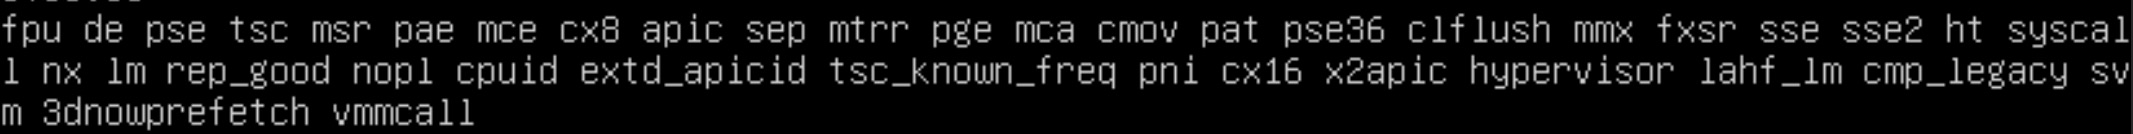
\includegraphics[width=1\textwidth]
    {assets/pics/lscpu_original.jpeg}
    \caption{Flag default KVM}
    \label{fig:lscpu_original}
\end{figure}

Terlihat pada gambar \ref{fig:lscpu_original} sama dengan Gambar \ref{fig:flag_kvm_host} di text yang ditebalkan. Dalam penelitian ini, flag yang akan diuji adalah \texttt{ssse3, sse4.1, sse4.2, sse4a, dan aes}. Semua flag SSE akan digunakan untuk percobaan kompresi video, sementara sse4.2 akan digunakan untuk validasi integritas file dengan CRC32, dan flag AES akan digunakan untuk enkripsi menggunakan AES. Harapannya, tuning ini akan memberikan peningkatan kinerja yang signifikan dibandingkan dengan konfigurasi default dari KVM.

Untuk melakukan tuning flag pada Hypervisor KVM, langkah pertama yang harus dilakukan adalah melihat daftar lengkap virtual machine yang sedang berjalan di sistem. Hal ini dapat dilakukan dengan menggunakan perintah:

\begin{lstlisting}
    virsh list
\end{lstlisting}

Keluaran dari perintah ini adalah:
\begin{figure}
    \centering
    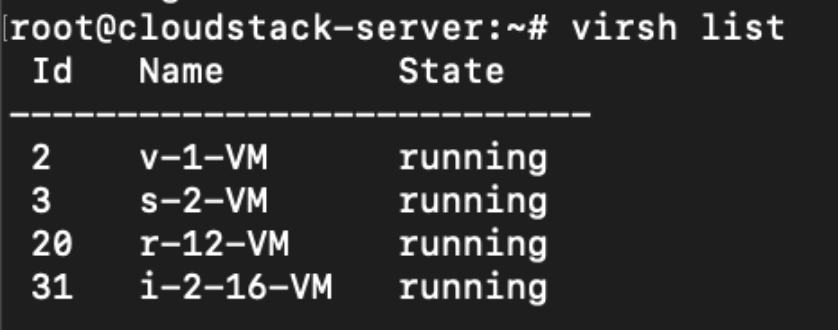
\includegraphics[width=0.5\textwidth]
    {assets/pics/virsh_list.png}
    \caption{Keluaran perintah \texttt{virsh list}}
    \label{fig:virsh_list}
\end{figure}

Pada Gambar \ref{fig:virsh_list} terlihat daftar virtual machine yang sedang berjalan di sistem. Dari daftar ini, virtual machine yang akan di-tuning adalah \texttt{i-2-16-VM}. Setelah mendapatkan nama virtual machine yang akan di-tuning (\texttt{i-2-16-VM}), gunakan perintah \texttt{virsh edit i-2-16-VM} untuk melihat konfigurasi virtual machine tersebut.

\begin{figure}
    \centering
    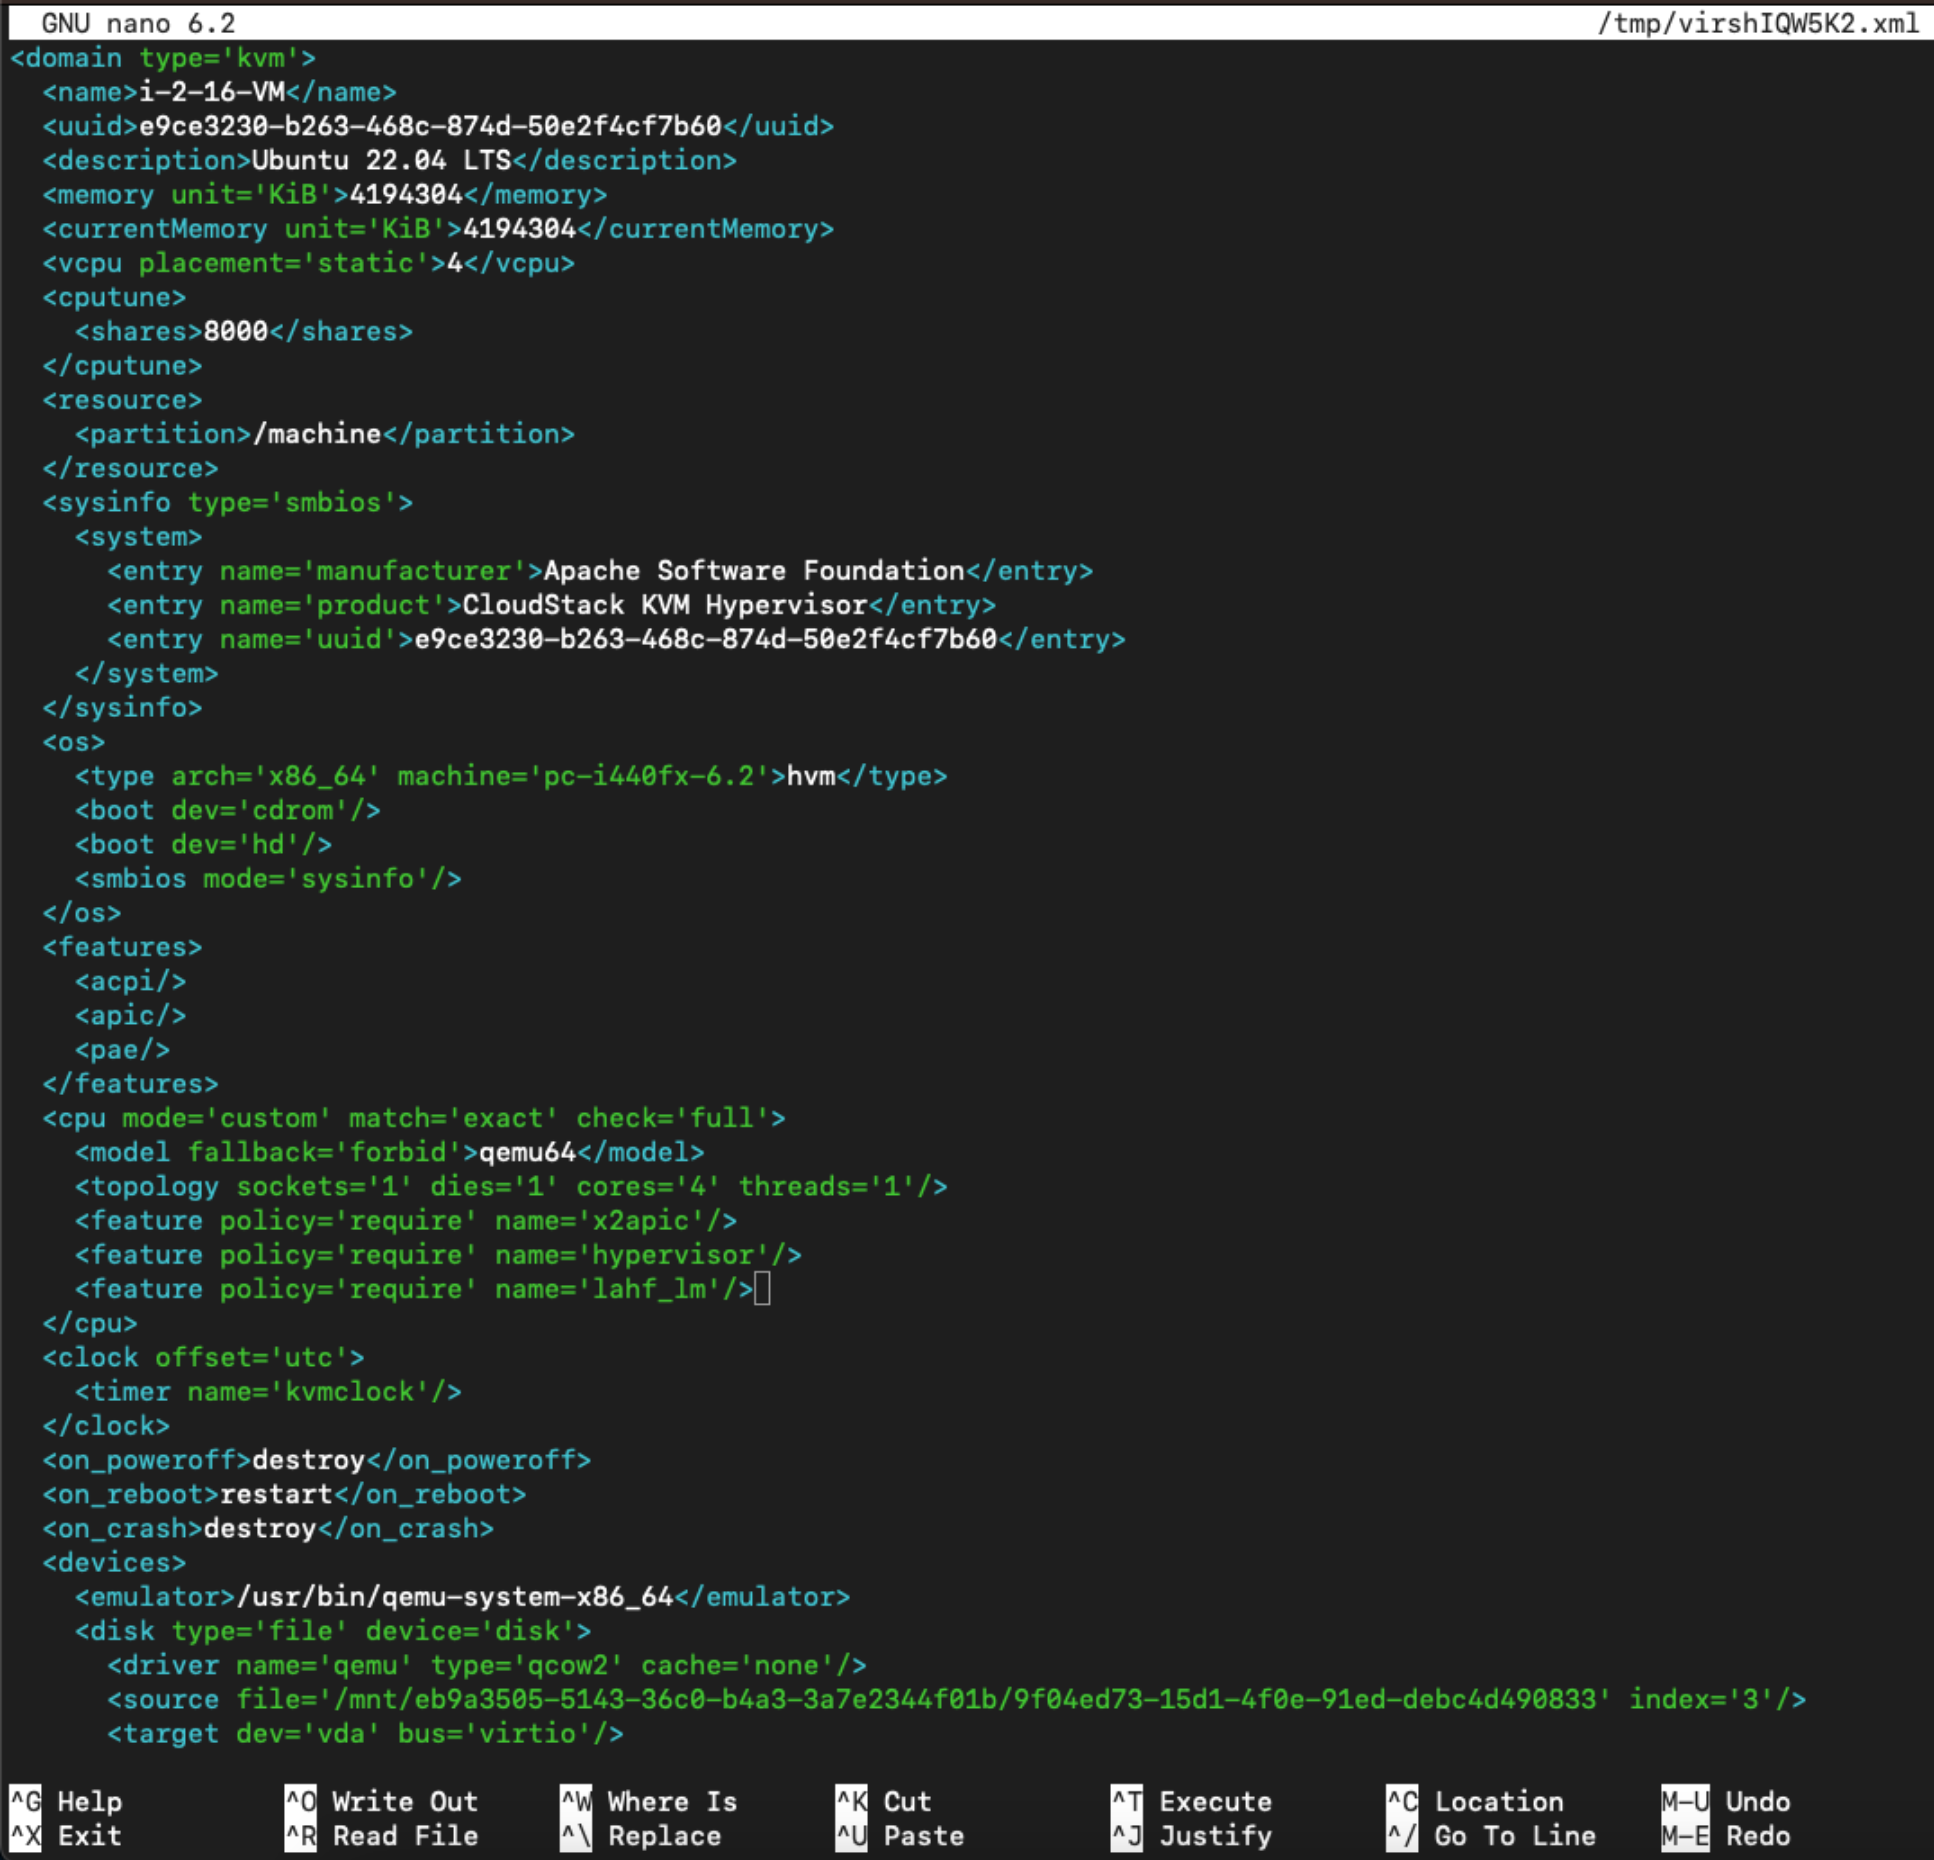
\includegraphics[width=0.9\textwidth]
    {assets/pics/virsh_edit1.png}
    \caption{Perintah \texttt{virsh edit i-2-16-VM} untuk melihat konfigurasi virtual machine \texttt{i-2-16-VM}}
    \label{fig:virsh_edit1}
\end{figure}

Pada gambar \ref{fig:virsh_edit1} terlihat konfigurasi virtual machine \texttt{i-2-16-VM}. Dari konfigurasi ini kita akan fokus pada bagian:

\begin{listing}[H]
    \begin{minted}{xml}
        ...

        <cpu mode='custom' match='exact' check='full'>
            <model fallback='forbid'>qemu64</model>
            <topology sockets='1' dies='1' cores='4' threads='1'/>
            <feature policy='require' name='x2apic'/>
            <feature policy='require' name='hypervisor'/> 
            <feature policy='require' name='lahf_1m'/>
        </cpu>
        
        ...
    \end{minted}
    \caption{Konfigurasi flag default}
    \label{code:default_kvm_xml}
\end{listing}

Kode \ref{code:default_kvm_xml} menampilkan konfigurasi flag default dari hypervisor KVM. Langkah berikutnya adalah menambahkan flag instruksi yang tidak termasuk dalam konfigurasi KVM default. Untuk melakukan ini, dilakukan duplikasi konfigurasi tersebut ke dalam sebuah file baru, seperti dalam penelitian ini yang akan disimpan di file \texttt{tuned\_kvm.xml}. Setelah disimpan di file \texttt{tuned\_kvm.xml}, selanjutnya dilakukan penambahan fitur yang diinginkan.

\begin{listing}[H]
    \begin{minted}{xml}
        ...

        <cpu mode='custom' match='exact' check='full'>
            <model fallback='forbid'>qemu64</model>
            <topology sockets='1' dies='1' cores='4' threads='1'/>
            <feature policy='require' name='x2apic'/>
            <feature policy='require' name='hypervisor'/> 
            <feature policy='require' name='lahf_1m'/>
            <feature policy='require' name='ssse3'/>
        </cpu>
        
        ...
    \end{minted}
    \caption{Konfigurasi flag ssse3}
    \label{code:ssse3_kvm_xml}
\end{listing}

Pada kode \ref{code:ssse3_kvm_xml}, fitur \texttt{ssse3} ditambahkan dengan menambahkan baris \texttt{<feature policy='require' name='ssse3'/>} pada kode tersebut. Setelah mengubah file \texttt{tuned\_kvm.xml}, simpan perubahan pada file tersebut. Selanjutnya, matikan mesin virtual dengan menggunakan perintah \texttt{destroy}:

\begin{lstlisting}
    virsh destroy i-2-16-VM
\end{lstlisting}

Setelah virtual machine dimatikan, langkah selanjutnya adalah membuat virtual machine baru berdasarkan konfigurasi yang telah diubah sebelumnya. Hal ini dapat dilakukan dengan menggunakan perintah:

\begin{lstlisting}
    virsh create tuned_kvm.xml
\end{lstlisting}

Dengan perintah ini maka \vm\ \texttt{i-2-16-VM} akan dibuat menggunakan konfigurasi \texttt{tuned\_kvm.xml}. Kita dapat melihat perubahan pada \vm\ \texttt{i-2-16-VM} dengan menggunakan perintah \texttt{lscpu} pada console virtual machine.

\begin{figure}
    \centering
    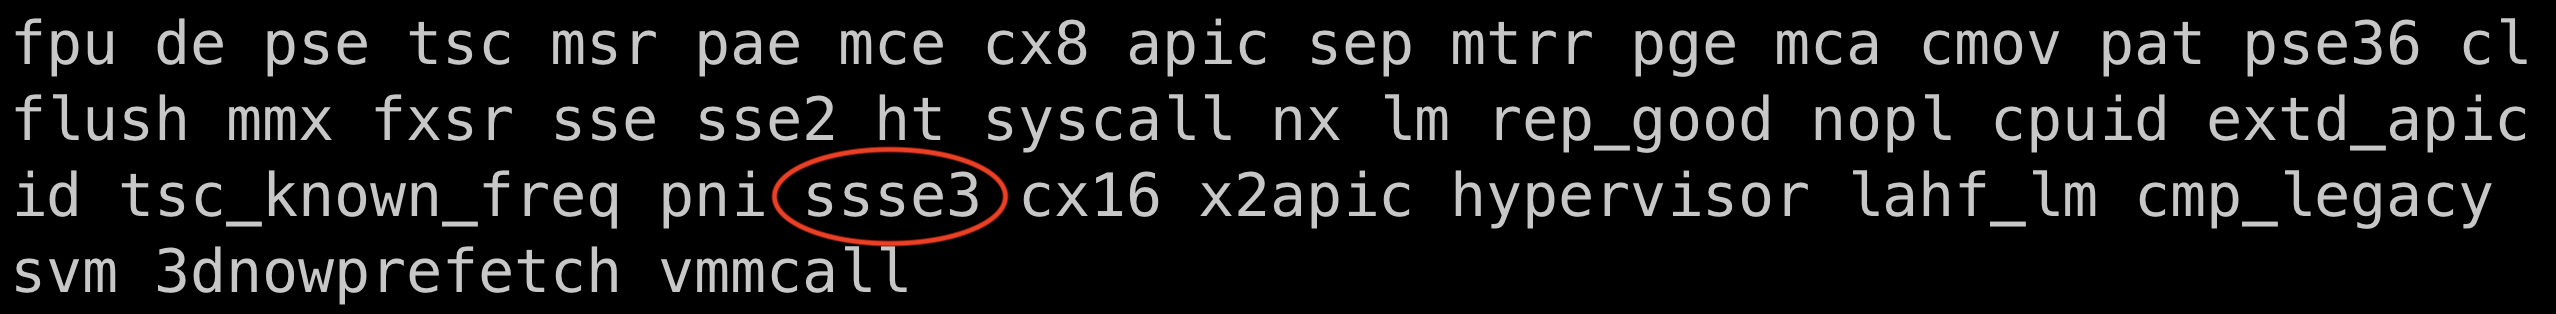
\includegraphics[width=1\textwidth]
    {assets/pics/lscpu_ssse3.jpeg}
    \caption{Flag tuned dengan ssse3}
    \label{fig:lscpu_ssse3}
\end{figure}

Dengan ini menandakan bahwa flag \texttt{ssse3} pada \vm\ \texttt{i-2-16-VM} sudah diaktifkan dan Hypervisor KVM sudah berhasil dituning.

%-----------------------------------------------------------------------------%
\subsection{Konfigurasi Hypervisor KVM untuk Kompresi Video}
%-----------------------------------------------------------------------------%
Pengujian kompresi video akan menggunakan konfigurasi seperti terlihat pada kode \ref{code:tuned_kompresi_video} yaitu dengan menggunakan flag ssse3, sse4.1, sse4.2, dan sse4a. Pemilihan flag-flag ini didasarkan pada instruksi SIMD (Single Instruction, Multiple Data) yang digunakan untuk operasi vektor pada data. Instruksi SIMD memungkinkan prosesor melakukan operasi secara bersamaan pada beberapa elemen data, sehingga mempercepat proses kompresi video dengan memanfaatkan kemampuan tersebut.

\begin{listing}[H]
    \begin{minted}{xml}
        ...

        <cpu mode='custom' match='exact' check='full'>
            <model fallback='forbid'>qemu64</model>
            <topology sockets='1' dies='1' cores='4' threads='1'/>
            <feature policy='require' name='x2apic'/>
            <feature policy='require' name='hypervisor'/> 
            <feature policy='require' name='lahf_1m'/>
            <feature policy='require' name='ssse3'/>
            <feature policy='require' name='sse4.1'/>
            <feature policy='require' name='sse4.2'/>
            <feature policy='require' name='sse4a'/>
        </cpu>
        
        ...
    \end{minted}
    \caption{Konfigurasi Hypervisor KVM untuk Kompresi Video}
    \label{code:tuned_kompresi_video}
\end{listing}

%-----------------------------------------------------------------------------%
\subsection{Konfigurasi Hypervisor KVM untuk Validasi Integritas File}
%-----------------------------------------------------------------------------%
Untuk melakukan pengujian dengan validasi integritas file akan digunakan konfigurasi seperti pada kode \ref{code:tuned_validasi_integritas_file}. Flag yang akan digunakan adalah sse4.2. Flag ini dipilih dikarenakan salah satu kemampuan yang dimiliki oleh flag ini adalah mendukung instruksi CRC32 yang akan digunakan untuk validasi integritas file.

\begin{listing}[H]
    \begin{minted}{xml}
        ...

        <cpu mode='custom' match='exact' check='full'>
            <model fallback='forbid'>qemu64</model>
            <topology sockets='1' dies='1' cores='4' threads='1'/>
            <feature policy='require' name='x2apic'/>
            <feature policy='require' name='hypervisor'/> 
            <feature policy='require' name='lahf_1m'/>
            <feature policy='require' name='sse4.2'/>
        </cpu>
        
        ...
    \end{minted}
    \caption{Konfigurasi Hypervisor KVM untuk Validasi Integritas File}
    \label{code:tuned_validasi_integritas_file}
\end{listing}

%-----------------------------------------------------------------------------%
\subsection{Konfigurasi Hypervisor KVM untuk Enkripsi AES}
%-----------------------------------------------------------------------------%
Untuk melakukan pengujian dengan enkripsi AES akan digunakan konfigurasi seperti pada kode \ref{code:tuned_enkripsi_aes}. Flag yang akan digunakan adalah aes. Flag ini dipilih dikarenakan salah satu kemampuan yang dimiliki oleh flag ini adalah mendukung instruksi AES yang akan digunakan untuk enkripsi AES.

\begin{listing}[H]
    \begin{minted}{xml}
        ...

        <cpu mode='custom' match='exact' check='full'>
            <model fallback='forbid'>qemu64</model>
            <topology sockets='1' dies='1' cores='4' threads='1'/>
            <feature policy='require' name='x2apic'/>
            <feature policy='require' name='hypervisor'/> 
            <feature policy='require' name='lahf_1m'/>
            <feature policy='require' name='aes'/>
        </cpu>
        
        ...
    \end{minted}
    \caption{Konfigurasi Hypervisor KVM untuk Enkripsi AES}
    \label{code:tuned_enkripsi_aes}
\end{listing}

%-----------------------------------------------------------------------------%
\section{Skenario Pengujian Tuning}
%-----------------------------------------------------------------------------%
Pada bagian ini akan dijelaskan skenario pengujian yang akan dilakukan untuk mengukur dampak tuning yang dilakukan pada Hypervisor KVM terhadap kinerja virtual machine. Pengujian akan dilakukan dengan menggunakan tiga skenario yang berbeda, yaitu kompresi video, validasi integritas file, dan enkripsi AES. Setiap skenario akan dijalankan pada virtual machine yang telah dituning dengan konfigurasi yang sesuai.

%-----------------------------------------------------------------------------%
\subsection{Skenario Pengujian Kompresi Video}
%-----------------------------------------------------------------------------%
Pada pengujian kompresi video akan dilakukan dengan menggunakan perangkat lunak ffmpeg untuk melakukan kompresi video. Pengujian ini akan mengukur waktu yang diperlukan untuk melakukan kompresi video dengan menggunakan konfigurasi tuning yang telah dilakukan pada Hypervisor KVM. Pengujian ini akan dilakukan dengan menggunakan video yang berjudul \texttt{Times Square Day Wide} yang memiliki durasi 10 detik dan resolusi 4k. Video ini akan dikompresi menggunakan codec h265 dengan preset medium. Pengujian akan dijalankan sebanyak 10 kali dan diukur waktu yang diperlukan untuk menyelesaikan proses kompresi video. Skrip bash yang digunakan untuk melakukan pengujian kompresi video dapat dilihat pada kode \ref{code:kode_pengujian_kompresi_video}.

\begin{listing}[H]
    \begin{minted}{bash}
    #!/bin/bash
    
    # Specify the path to your input video file
    input_file="timessquaredaywide.mp4"

    # Specify the output directory
    output_directory="output"

    # Specify the number of times to run the benchmark
    num_runs=10

    # Loop to run the benchmark command multiple times
    for i in $(seq 1 $num_runs)
    do
        start_time=$(date +%s.%N)
        log_file="$output_directory/log_$i.txt"
        
        echo "Running benchmark $i..."
        
        # Add your ffmpeg compression command here
        ffmpeg -i "$input_file" -c:v libx265 -preset medium -crf 32 -c:a aac -strict -2 "$output_directory/output_$i.mp4" > "$log_file" 2>&1
        
        end_time=$(date +%s.%N)
        elapsed_time=$(awk "BEGIN {print $end_time - $start_time}")
        
        echo "Benchmark $i completed in $elapsed_time seconds. Log saved to $log_file."
    done
    \end{minted}
    \caption{Kode Pengujian Kompresi Video}
    \label{code:kode_pengujian_kompresi_video}
\end{listing}

%-----------------------------------------------------------------------------%
\subsection{Skenario Pengujian Validasi Integritas File}
%-----------------------------------------------------------------------------%
Pada pengujian validasi integritas file akan dilakukan dengan menggunakan library crc32c dari python untuk melakukan perhitungan CRC32 pada file. Pengujian ini akan mengukur waktu yang diperlukan untuk melakukan perhitungan CRC32 pada file dengan ukuran 10 MB. Pengujian ini akan dijalankan sebanyak 10 kali dan diukur waktu yang diperlukan untuk menyelesaikan proses perhitungan CRC32. Skrip python yang digunakan untuk melakukan pengujian validasi integritas file dapat dilihat pada kode \ref{code:kode_pengujian_validasi_integritas_file}.

\begin{listing}[H]
    \begin{minted}{python}
    import os
    import time
    import crc32c

    def benchmark_crc32c(data, iterations):
        # Perform CRC32 calculation
        start_time = time.time()
        for _ in range(iterations):
            crc32c.crc32c(data)
        end_time = time.time()

        # Calculate average time per iteration
        avg_time = (end_time - start_time) / iterations
        return avg_time

    def main(i):
        # Define parameters
        data_size = 10 * 1024 * 1024  # Size of the data (10 MB)
        num_iterations = 1000  # Number of iterations to average the time

        # Generate random data
        data = bytearray(os.urandom(data_size))

        # Run the benchmark
        avg_time_crc32c = benchmark_crc32c(data, num_iterations)
        print(
            f"Run {i + 1} Average time for CRC32 calculation: {avg_time_crc32c * 1000} ms"
        )

    for i in range(10):
        main(i)

    \end{minted}
    \caption{Kode Pengujian Validasi Integritas File}
    \label{code:kode_pengujian_validasi_integritas_file}
\end{listing}

%-----------------------------------------------------------------------------%
\subsection{Skenario Pengujian Enkripsi AES}
%-----------------------------------------------------------------------------%
Pada pengujian enkripsi AES akan dilakukan dengan menggunakan library cryptography dari python untuk melakukan enkripsi AES. Pengujian ini akan mengukur waktu yang diperlukan untuk melakukan enkripsi AES pada data teks Gambar \ref{fig:aesPlaintextData}. Pengujian ini akan dijalankan sebanyak 10 kali dan diukur waktu yang diperlukan untuk menyelesaikan proses enkripsi AES. Skrip python yang digunakan untuk melakukan pengujian enkripsi AES dapat dilihat pada kode \ref{code:pengujian_enkripsi_aes_1} dan \ref{code:pengujian_enkripsi_aes_2}.

\begin{figure}
    \begin{lstlisting}
The Advanced Encryption Standard (AES) is a symmetric-key encryption algorithm that has become the de facto standard for securing sensitive data worldwide. Developed by Belgian cryptographers Joan Daemen and Vincent Rijmen, AES was adopted by the U.S. National Institute of Standards and Technology (NIST) in 2001 after a rigorous evaluation process involving numerous submissions from around the globe. AES replaced the aging Data Encryption Standard (DES) and its variants, which were becoming increasingly vulnerable to brute-force attacks due to advances in computing power.
...
AES has been extensively studied and scrutinized by cryptographers worldwide, and its strength lies in its ability to withstand known attacks while maintaining high performance. Consequently, AES has been widely adopted in various industries, including government, finance, healthcare, and telecommunications, as well as in protocols and standards such as TLS/SSL, IPsec, and wireless encryption standards like WPA2.
    \end{lstlisting}
    \caption{Potongan Plaintext Data untuk AES Encryption Benchmark}
    \label{fig:aesPlaintextData}
\end{figure}

%  AES operates on fixed block sizes of 128 bits and supports key lengths of 128, 192, or 256 bits, with the latter providing the highest level of security. Its sophisticated mathematical structure, based on substitution-permutation networks, makes it highly resistant to various cryptanalytic attacks, including differential and linear cryptanalysis. AES employs multiple rounds of substitution, permutation, and key mixing operations to scramble the plaintext data, making it virtually impossible to decrypt without the correct key. One of the key strengths of AES is its versatility and flexibility. It can be implemented in hardware or software, making it suitable for a wide range of applications, from securing communication channels to protecting data at rest.

\begin{listing}[H]
    \begin{minted}{python}
    from cryptography.hazmat.primitives.ciphers import Cipher, algorithms, modes
    from cryptography.hazmat.primitives import padding
    from cryptography.hazmat.backends import default_backend
    import time

    # Generate a random AES key and plaintext
    key = b"sixteenbytekey12"
    plaintext = # Gambar Potongan Plaintext Data untuk AES Encryption Benchmark

    # Function to perform AES encryption benchmark
    def aes_encrypt_benchmark(key, plaintext):
        backend = default_backend()
        cipher = Cipher(algorithms.AES(key), modes.ECB(), backend=backend)
        encryptor = cipher.encryptor()

        padder = padding.PKCS7(algorithms.AES.block_size).padder()
        padded_plaintext = padder.update(plaintext) + padder.finalize()

        start_time = time.time()
        ciphertext = encryptor.update(padded_plaintext) + encryptor.finalize()
        end_time = time.time()

        return ciphertext, end_time - start_time

    # Function to perform AES decryption benchmark
    def aes_decrypt_benchmark(key, ciphertext):
        backend = default_backend()
        cipher = Cipher(algorithms.AES(key), modes.ECB(), backend=backend)
        decryptor = cipher.decryptor()

        start_time = time.time()
        padded_plaintext = decryptor.update(ciphertext) + decryptor.finalize()
        end_time = time.time()

        unpadder = padding.PKCS7(algorithms.AES.block_size).unpadder()
        plaintext = unpadder.update(padded_plaintext) + unpadder.finalize()

        return end_time - start_time
    \end{minted}
    \caption{Kode Pengujian Enkripsi AES (1)}
    \label{code:pengujian_enkripsi_aes_1}
\end{listing}

\begin{listing}[H]
    \begin{minted}{python}
    def run_benchmark():
        # Benchmark AES encryption
        ciphertext, aes_time_encrypt = aes_encrypt_benchmark(key, plaintext)
        # print(f"AES Encryption Time: {(aes_time_encrypt * 1000):.5f} ms")

        # Benchmark AES decryption
        aes_time_decrypt = aes_decrypt_benchmark(key, ciphertext)
        # print(f"AES Decryption Time: {(aes_time_decrypt * 1000):.5f} ms")
        return aes_time_encrypt, aes_time_decrypt

    def main(i):
        iterations = 1000

        encrypt_time = 0
        decrypt_time = 0
        for _ in range(iterations):
            encrypt_time_iter, decrypt_time_iter = run_benchmark()
            encrypt_time += encrypt_time_iter
            decrypt_time += decrypt_time_iter

        avg_encrypt_time = encrypt_time / iterations
        avg_decrypt_time = decrypt_time / iterations

        print(f"Run {i+1} Average AES Encryption Time: {(avg_encrypt_time * 1000):.5f} ms")
        print(
            f"Run {i+1} Average AES Decryption Time: {(avg_decrypt_time * 1000):.5f} ms\n"
        )

    for i in range(10):
        main(i)

    \end{minted}
    \caption{Kode Pengujian Enkripsi AES (2)}
    \label{code:pengujian_enkripsi_aes_2}
\end{listing}
%-----------------------------------------------------------------------------%
\section{Analisis}
%-----------------------------------------------------------------------------%
Analisis akan dilakukan dengan melakukan perhitungan menggunakan formula \texttt{speedup}. Diasumsikan bahwa T(1) adalah waktu eksekusi Test dengan konfigurasi default, dan T(p) adalah waktu eksekusi Test dengan konfigurasi yang telah dituning\cite{beuwolfCetin}.

Formula \texttt{speedup} dinyatakan sebagai berikut:

\begin{equation}
    S(p) = \frac{T(1)}{T(p)} 
    \label{eq:formula}
\end{equation}

Berdasarkan rumus \ref{eq:formula}, jika nilai S(p) semakin besar, maka konfigurasi yang dituning semakin bagus. Hal ini menandakan bahwa tuning Hypervisor dapat mempercepat proses yang dilakukan. Sebaliknya, jika S(p) semakin kecil, maka konfigurasi yang dituning semakin lambat. Jika nilai S(p) sama, maka efek dari konfigurasi yang dituning sama dengan konfigurasi default.

%-----------------------------------------------------------------------------%
\subsection{Analisis Pengujian Kompresi Video}
%-----------------------------------------------------------------------------%
Dalam analisis pengujian dengan kompresi video, akan dibandingkan waktu eksekusi antara konfigurasi Hypervisor yang tidak dituning (default) dan konfigurasi yang telah dituning. Perbandingan ini dilakukan dengan menggunakan formula \texttt{speedup}. Konfigurasi yang optimal adalah konfigurasi yang memiliki nilai \texttt{speedup} tertinggi, yang menunjukkan peningkatan kinerja yang signifikan dalam proses kompresi video.

%-----------------------------------------------------------------------------%
\subsection{Analisis Pengujian Validasi Integritas File}
%-----------------------------------------------------------------------------%
Untuk analisis pengujian validasi integritas file, akan digunakan pendekatan yang serupa dengan analisis kompresi video. Akan dibandingkan waktu eksekusi antara konfigurasi Hypervisor yang tidak dituning (default) dan konfigurasi yang telah dituning menggunakan formula \texttt{speedup}. Nilai S(p) yang lebih besar menunjukkan bahwa konfigurasi yang dituning lebih efisien dalam memverifikasi integritas file dibandingkan dengan konfigurasi default. Konfigurasi yang optimal adalah konfigurasi yang memiliki nilai \texttt{speedup} tertinggi, yang mengindikasikan peningkatan kinerja yang signifikan dalam proses validasi integritas file.

%-----------------------------------------------------------------------------%
\subsection{Analisis Pengujian Enkripsi AES}
%-----------------------------------------------------------------------------%
Dalam analisis pengujian enkripsi AES, kami akan menggunakan metode yang sama seperti analisis sebelumnya, yaitu dengan membandingkan waktu eksekusi antara konfigurasi Hypervisor yang tidak dituning (default) dan konfigurasi yang telah dituning menggunakan formula \texttt{speedup}. Nilai S(p) yang lebih besar menunjukkan bahwa konfigurasi yang dituning lebih efisien dalam melakukan enkripsi AES dibandingkan dengan konfigurasi default. Konfigurasi yang optimal adalah konfigurasi yang memiliki nilai \texttt{speedup} tertinggi, yang mengindikasikan peningkatan kinerja yang signifikan dalam proses enkripsi AES.

\hfill

Dengan menganalisis nilai \texttt{speedup}, kami dapat mengevaluasi dan membandingkan kinerja berbagai konfigurasi Hypervisor dalam melakukan tugas-tugas seperti kompresi video, validasi integritas file, dan enkripsi AES. Konfigurasi dengan nilai \texttt{speedup} tertinggi akan menjadi pilihan yang optimal untuk meningkatkan kinerja dan efisiensi dalam setiap tugas yang diuji.

\iffalse
    %-----------------------------------------------------------------------------%
    \section{Pengujian Kompresi Video Dengan HandBrake}
    %-----------------------------------------------------------------------------%
    Untuk menguji dan membandingkan kinerja Hypervisor KVM sebelum dan sesudah tuning, {\saya} akan menggunakan software HandBrake, sebuah software kompresi video yang sudah banyak digunakan. Proses ini melibatkan penggunaan HandBrake untuk kompresi video pada dua lingkungan \vm\ yang berbeda, yang mana satu menggunakan KVM yang belum di-tuning dan yang lainnya menggunakan KVM yang telah di-tuning. Tujuan dari pengujian ini adalah untuk mengevaluasi sejauh mana tuning Hypervisor KVM dapat mempengaruhi kecepatan kompresi video.

    HandBrake dipilih karena kemampuannya yang baik dalam mengkompresi video dan mudah untuk digunakan\cite{Folgar2014eg}. Dalam pengujian ini, video yang akan digunakan adalah "COSTA RICA IN 4K 60fps HDR (ULTRA HD)" yang diunduh dari YouTube dengan resolusi video yang digunakan adalah 2K. Video ini dipilih karena resolusi tingginya, yang memberikan tantangan yang baik untuk menguji efisiensi kompresi video pada kedua lingkungan \vm.

    Parameter penting yang akan diukur dalam pengujian ini adalah:

    \begin{enumerate}
        \item \textbf{\f{Time Elapsed}}

              \f{Time Elapsed} atau berapa lama waktu yang dibutuhkan oleh masing-masing \vm\ untuk menyelesaikan proses kompresi video.

        \item \textbf{\f{Structural Similarity Index Measure Score}}

              Structural Similarity Index Measure adalah cara untuk menilai kesamaan dari 2 buah gambar, untuk melihat apakah terjadi penurunan kualitas atau perbedaan yang besar antara gambar yang belum di compress dengan gambar yang sudah di compress.
    \end{enumerate}


    Data ini yang akan memberikan gambaran yang jelas mengenai perbedaan kinerja antara KVM yang telah di-tuning dengan yang belum.

    Spesifikasi dari \vm\ yang akan digunakan dalam pengujian ini adalah sebagai berikut:
    \begin{itemize}
        \item \textbf{Cloud Platform}: Apache CloudStack 4.18.1
        \item \textbf{OS}: Ubuntu Server 22.04 LTS
        \item \textbf{CPU}: 1 CPU x 1.00 Ghz
        \item \textbf{Memory}: 1024 MB
    \end{itemize}

    Perintah yang digunakan untuk melakukan kompresi video dengan handbrake adalah sebagai berikut:

    \begin{verbatim}
    ./HandBrakeCLI -i /path/to/input.mov -o /path/to/output.mp4
    -e x264 -q 28 -r 15 -B 64 -X 1280 -O
\end{verbatim}

    Dengan perintah ini \saya akan melakukan kompresi video dengan codec x264. Codec yang dikembangkan oleh VideoLAN yang sudah banyak digunakan dikarenakan mampu untuk melakukan kompresi video yang baik dan rendahnya tingkat penurunan kualitas gambar.

    %-----------------------------------------------------------------------------%
    \section{Analisis Pengujian}
    %-----------------------------------------------------------------------------%
    Dalam analisis ini, waktu kompresi untuk Hypervisor KVM yang belum di-tuning akan disebut sebagai $T_{\mathrm{default}}$, sementara waktu kompresi untuk Hypervisor KVM yang telah di-tuning akan disebut sebagai $T_{\mathrm{tuned}}$. Waktu kompresi ini akan diambil dari logs HandBrake yang telah melakukan kompresi video. Untuk mengetahui apakah terdapat perbedaan yang signifikan, \saya\ dapat menggunakan formula speedup.

    \[ \mathrm{Speedup} = \frac{T_{\mathrm{default}}}{T_{\mathrm{tuned}}} \]

    Jika nilai speedup lebih dari 1, ini menandakan bahwa proses kompresi dengan Hypervisor KVM yang sudah di-tuning lebih cepat dibandingkan dengan yang belum di-tuning.

    Pengujian akan dilakukan sebanyak kurang lebih sepuluh kali dan nantinya akan ditampilkan dalam bentuk grafik. Akan terdapat grafik \f{line chart} dengan dua garis dimana masing-merepresentasikan $T_{\mathrm{default}}$ dan $T_{\mathrm{tuned}}$.

    Selain menganalisis waktu kompresi video, \saya\ juga akan melakukan analisis untuk menilai kualitas video yang telah dikompresi. Analisis ini akan melibatkan perbandingan nilai dari \f{Structural Similarity Index Measure} (SSIM) antara video yang dikompres menggunakan Hypervisor KVM default dan Hypervisor KVM yang telah di-tuning. SSIM adalah metrik yang mengukur kesamaan visual antara dua video. Semakin tinggi nilai SSIM, semakin mirip video yang dikompres dengan versi aslinya. Oleh karena itu, nilai SSIM yang lebih tinggi menunjukkan kualitas kompresi yang lebih baik, dimana integritas visual dari video asli lebih terjaga.


    \iffalse
        Selanjutnya, \saya\ akan menghitung efisiensi dari tuning Hypervisor KVM ini. Untuk mengetahui efisiensi, \saya\ dapat menggunakan formula efisiensi.

        \[ \mathrm{Efficiency} = \frac{\mathrm{Speedup}}{\frac{R_{\mathrm{tuned}}}{R_{\mathrm{default}}}} \]


        Tujuan menghitung efisiensi ini adalah untuk mengetahui seberapa efektif tuning dilakukan dalam menggunakan sumber daya yang ada, seperti penggunaan CPU dan memori. Perhitungan ini penting untuk menilai kinerja tuning dalam konteks keseluruhan penggunaan sumber daya, tidak hanya kecepatan kompresi.
    \fi

    % Time Measurement
    %$T_{\mathrm{default}}$, $T_{\mathrm{tuned}}$
    %\[ T_{\mathrm{default}}, \quad T_{\mathrm{tuned}} \]

    % Speedup
    %$\mathrm{Speedup} = \frac{T_{\mathrm{default}}}{T_{\mathrm{tuned}}}$
    %\[ \mathrm{Speedup} = \frac{T_{\mathrm{default}}}{T_{\mathrm{tuned}}} \]



    %-----------------------------------------------------------------------------%
    \section{Satu Persamaan}
    %-----------------------------------------------------------------------------%

    \noindent \begin{align}\label{eq:garis}
        \cfrac{y - y_{1}}{y_{2} - y_{1}} =
        \cfrac{x - x_{1}}{x_{2} - x_{1}}
    \end{align}

    \equ~\ref{eq:garis} diatas adalah persamaan garis.
    \equ~\ref{eq:garis} dan \ref{eq:bola} sama-sama dibuat dengan perintah \bslash
    align.
    Perintah ini juga dapat digunakan untuk menulis lebih dari satu persamaan.

    \noindent \begin{align}\label{eq:bola}
        \underbrace{|\overline{ab}|}_{\text{pada bola $|\overline{ab}| = r$}}
        = \sqrt[2]{(x_{b} - x_{a})^{2} + (y_{b} - y_{a})^{2} +
            \vert\vert(z_{b} - z_{a})^{2}}
    \end{align}

    %-----------------------------------------------------------------------------%
    \section{Lebih dari Satu Persamaan}
    \label{sec:multiEqu}
    %-----------------------------------------------------------------------------%
    \noindent \begin{align}\label{eq:matriks}
        |\overline{a} * \overline{b}| & = |\overline{a}| |\overline{b}| \sin\theta
        \\[0.2cm]
        \overline{a} * \overline{b}   & =
        \begin{array}{| c c c |}
            \hat{i} & x_{1} & x_{2} \\
            \hat{j} & y_{1} & y_{2} \\
            \hat{k} & z_{1} & z_{2} \\
        \end{array} \nonumber                                                    \\[0.2cm]
                                      & = \hat{i} \,
        \begin{array}{ | c c | }
            y_{1} & y_{2} \\
            z_{1} & z_{2} \\
        \end{array}
        + \hat{j} \,
        \begin{array}{ | c c | }
            z_{1} & z_{2} \\
            x_{1} & x_{2} \\
        \end{array}
        + \hat{k} \,
        \begin{array}{ | c c | }
            x_{1} & x_{2} \\
            y_{1} & y_{2} \\
        \end{array}
        \nonumber
    \end{align}

    Pada \equ~\ref{eq:matriks} dapat dilihat beberapa baris menjadi satu bagian
    dari \equ~\ref{eq:matriks}.
    Sedangkan dibawah ini dapat dilihat bahwa dengan cara yang sama, \equ~
    \ref{eq:gabungan1}, \ref{eq:gabungan2}, dan \ref{eq:gabungan3} memiliki nomor
    persamaannya masing-masing.

    \noindent \begin{align}\label{eq:gabungan1}
        \int_{a}^{b} f(x)\, dx + \int_{b}^{c} f(x) \, dx = \int_{a}^{c} f(x) \, dx
        \\\label{eq:gabungan2}
        \lim_{x \to \infty} \frac{f(x)}{g(x)} = 0 \hspace{1cm}
        \text{jika pangkat $f(x)$ $<$ pangkat $g(x)$} \\\label{eq:gabungan3}
        a^{m^{a \, ^{n}\log b }} = b^{\frac{m}{n}}
    \end{align}
\fi

%\iffalse
%-----------------------------------------------------------------------------%
%\chapter{\babEmpat}
%-----------------------------------------------------------------------------%
\todo{tambahkan kata-kata pengantar bab 1 disini}

%-----------------------------------------------------------------------------%
\section{thesis.tex}
%-----------------------------------------------------------------------------%
Berkas ini berisi seluruh berkas Latex yang dibaca, jadi bisa dikatakan sebagai 
berkas utama. Dari berkas ini kita dapat mengatur bab apa saja yang ingin 
kita tampilkan dalam dokumen.


%-----------------------------------------------------------------------------%
\section{laporan\_setting.tex}
%-----------------------------------------------------------------------------%
Berkas ini berguna untuk mempermudah pembuatan beberapa template standar. 
Anda diminta untuk menuliskan judul laporan, nama, npm, dan hal-hal lain yang 
dibutuhkan untuk pembuatan template. 


%-----------------------------------------------------------------------------%
\section{istilah.tex}
%-----------------------------------------------------------------------------%
Berkas istilah digunakan untuk mencatat istilah-istilah yang digunakan. 
Fungsinya hanya untuk memudahkan penulisan.
Pada beberapa kasus, ada kata-kata yang harus selalu muncul dengan tercetak 
miring atau tercetak tebal. 
Dengan menjadikan kata-kata tersebut sebagai sebuah perintah \latex~tentu akan 
mempercepat dan mempermudah pengerjaan laporan. 


%-----------------------------------------------------------------------------%
\section{hype.indonesia.tex}
%-----------------------------------------------------------------------------%
Berkas ini berisi cara pemenggalan beberapa kata dalam bahasa Indonesia. 
\latex~memiliki algoritma untuk memenggal kata-kata sendiri, namun untuk 
beberapa kasus algoritma ini memenggal dengan cara yang salah. 
Untuk memperbaiki pemenggalan yang salah inilah cara pemenggalan yang benar 
ditulis dalam berkas hype.indonesia.tex.


%-----------------------------------------------------------------------------%
\section{pustaka.tex}
%-----------------------------------------------------------------------------%
Berkas pustaka.tex berisi seluruh daftar referensi yang digunakan dalam 
laporan. 
Anda bisa membuat model daftar referensi lain dengan menggunakan bibtex.
Untuk mempelajari bibtex lebih lanjut, silahkan buka 
\url{http://www.bibtex.org/Format}. 
Untuk merujuk pada salah satu referensi yang ada, gunakan perintah \bslash 
cite, e.g. \bslash cite\{lankton2008introduction\} yang akan akan memunculkan 
\cite{lankton2008introduction}


%-----------------------------------------------------------------------------%
\section{bab[1 - 6].tex}
%-----------------------------------------------------------------------------%
Berkas ini berisi isi laporan yang Anda tulis. 
Setiap nama berkas e.g. bab1.tex merepresentasikan bab dimana tulisan tersebut 
akan muncul. 
Sebagai contoh, kode dimana tulisan ini dibaut berada dalam berkas dengan nama 
bab4.tex. 
Ada enam buah berkas yang telah disiapkan untuk mengakomodir enam bab dari 
laporan Anda, diluar bab kesimpulan dan saran. 
Jika Anda tidak membutuhkan sebanyak itu, silahkan hapus kode dalam berkas 
thesis.tex yang memasukan berkas \latex~yang tidak dibutuhkan;  contohnya 
perintah \bslash include\{bab6.tex\} merupakan kode untuk memasukan berkas 
bab6.tex kedalam laporan.

%-----------------------------------------------------------------------------%
\section{Penulisan \textit{code} atau \textit{pseudocode} program}
%-----------------------------------------------------------------------------%

\subsection{\textit{Inline}}

Dengan perintah \verb|\verb|: \verb|System.out.println("Hello, World");| \\
Dengan perintah \textit{custom} \verb|\code|: \code{System.out.println("Hello, World"); }
Dengan perintah \verb|\mintinline|: \mintinline{java}{System.out.println("Hello, World"); }

\subsection{\textit{Multiline}}

Dengan perintah \verb|verbatim|: 

\begin{verbatim}	
public class HelloWorld {
    public static void main(String[] args) {
        // Prints "Hello, World" to the terminal window.
        System.out.println("Hello, World");
    }
}
\end{verbatim}

Dengan perintah \verb|minted|: Kode \ref{code:hw:minted}
\begin{listing}[H]
    \begin{minted}{python}
def binary_accuracy(y_true, y_pred):
    return K.mean(K.equal(y_true, K.round(y_pred)), axis=-1)


def categorical_accuracy(y_true, y_pred):
    return K.cast(K.equal(K.argmax(y_true, axis=-1),
                          K.argmax(y_pred, axis=-1)),
                  K.floatx())


def sparse_categorical_accuracy(y_true, y_pred):
    # reshape in case it's in shape (num_samples, 1) instead of (num_samples,)
    if K.ndim(y_true) == K.ndim(y_pred):
        y_true = K.squeeze(y_true, -1)
    # convert dense predictions to labels
    y_pred_labels = K.argmax(y_pred, axis=-1)
    y_pred_labels = K.cast(y_pred_labels, K.floatx())
    return K.cast(K.equal(y_true, y_pred_labels), K.floatx())


def top_k_categorical_accuracy(y_true, y_pred, k=5):
    return K.mean(K.in_top_k(y_pred, K.argmax(y_true, axis=-1), k), axis=-1)


def sparse_top_k_categorical_accuracy(y_true, y_pred, k=5):
    # If the shape of y_true is (num_samples, 1), flatten to (num_samples,)
    return K.mean(K.in_top_k(y_pred, K.cast(K.flatten(y_true), 'int32'), k),
                  axis=-1)
    \end{minted}
    \caption{An excerpt from keras: \url{https://github.com/keras-team/keras/blob/master/keras/metrics.py}}
    \label{code:hw:minted}
\end{listing}

Konfigurasi tampilan bisa dilakukan di \verb|uithesis.sty| dengan referensi dokumentasi di \url{https://github.com/gpoore/minted/blob/master/source/minted.pdf}

\fi
%%-----------------------------------------------------------------------------%
\chapter{\babLima}
%-----------------------------------------------------------------------------%

Berdasarkan hasil pengujian hasil tuning hypervisor dari tiga skenario berbeda yang telah dilakukan, dapat disimpulkan berbagai hal:

\begin{enumerate}
	\item Flag default yang disediakan oleh hypervisor bersifat minimal, sehingga perlu dilakukan tuning untuk meningkatkan performa sesuai dengan kebutuhan dari pengguna.
	\item Dari hasil pengujian tuning hypervisor dengan kompresi video dengan menggunakan tools ffmpeg, kombinasi feature flag yang paling baik untuk digunakan adalah SSSE3 dan SSE4.1 dengan kecepatan kompresi video sebesar 2.43 kali lebih cepat dibandingkan dengan flag default.
	\item Dari hasil pengujian tuning hypervisor dengan validasi integritas data menggunakan fungsu CRC32, penambahan feature flag sse4.2 dapat mempercepat proses validasi integritas file sebesar 7.68 kali lebih cepat dibandingkan dengan flag default.
	\item Dari hasil pengujian tuning hypervisor dengan enkrispi AES, penambahan feature flag aes dapat mempercepat proses enkripsi AES sebesar 2.17 kali lebih cepat dibandingkan dengan flag default.
	\item Dari hasil pengujian tuning hypervisor dengan dekripsi AES, penambahan feature flag aes dapat mempercepat proses dekripsi AES sebesar 2.68 kali lebih cepat dibandingkan dengan flag default.
	\item Dengan melakukan tuning hypervisor yang tepat, performa dalam menjalankan aplikasi dapat ditingkatkan sesuai dengan kebutuhan pengguna.
\end{enumerate}

%-----------------------------------------------------------------------------%
\section{Saran}
%-----------------------------------------------------------------------------%
Setelah dilakukan penelitian dan pengujian terhadap tuning hypervisor untuk \vm\ di Apache Cloudstack, \saya\ menemukan beberapa sayran yang bisa menjadi pertimbangan untuk meningkatkan penelitian pada topik ini kedepannya:

\begin{itemize}
	\item Menggunakan jenis CPU yang berbeda untuk melakukan tuning hypervisor, karena setiap jenis CPU memiliki karakteristik dan fungsi yang berbeda.
	\item Melakukan evaluasi pengaruh tuning hypervisor terhadap kinerja aplikasi yang berbeda, misalnya, aplikasi web, basis data, atau aplikasi real-time.
	\item Memberikan contoh kasus penggunaan yang lebih kompleks, seperti penggunaan hypervisor untuk kebutuhan \textit{machine learning} atau \textit{big data} dan menganalisis efek dari tuning hypervisor pada kasus tersebut.
	\item Untuk konteks penelitian tuning hypervisor, dapat digunakan jenis Cloud Management Platform (CMP) yang berbeda, seperti OpenStack, ManageIQ, atau Cloudify.
	\item Membandingkan efektivitas tuning hypervisor pada lingkungan virtualisasi yang berbeda, seperti (\textit{full virtualization}), paravirtualisasi, atau kontainerisasi.
	\item Menggunakan flag AVX/AVX2 untuk melakukan pengujian tuning dengan kompresi video. Dikarenakan AVX merupakan flag pembaruan dari SSE.
\end{itemize}

\iffalse
	%-----------------------------------------------------------------------------%
	\section{Mengubah Tampilan Teks}
	%-----------------------------------------------------------------------------%
	Beberapa perintah yang dapat digunakan untuk mengubah tampilan adalah:
	\begin{itemize}
		\item \bslash f \\
		      Merupakan alias untuk perintah \bslash textit, contoh
		      \f{contoh hasil tulisan}.
		\item \bslash bi \\
		      \bi{Contoh hasil tulisan}.
		\item \bslash bo \\
		      \bo{Contoh hasil tulisan}.
		\item \bslash m \\
		      Contoh\ hasil\ tulisan: $\alpha \not= \m{\alpha}$
		\item \bslash code \\
		      \code{Contoh hasil tulisan}.
	\end{itemize}


	%-----------------------------------------------------------------------------%
	\section{Memberikan Catatan}
	%-----------------------------------------------------------------------------%
	Ada dua perintah untuk memberikan catatan penulisan dalam dokumen yang Anda
	kerjakan, yaitu:
	\begin{itemize}
		\item \bslash todo \\
		      Contoh: \\ \todo{Contoh bentuk todo.}
		\item \bslash todoCite \\
		      Contoh: \todoCite
	\end{itemize}


	%-----------------------------------------------------------------------------%
	\section{Menambah Isi Daftar Isi}
	%-----------------------------------------------------------------------------%
	Terkadang ada kebutuhan untuk memasukan kata-kata tertentu kedalam Daftar Isi.
	Perintah \bslash addChapter dapat digunakan untuk judul bab dalam Daftar isi.
	Contohnya dapat dilihat pada berkas thesis.tex.


	%-----------------------------------------------------------------------------%
	\section{Memasukan PDF}
	%-----------------------------------------------------------------------------%
	Untuk memasukan PDF dapat menggunakan perintah \bslash inpdf yang menerima satu
	buah argumen. Argumen ini berisi nama berkas yang akan digabungkan dalam
	laporan. PDF yang dimasukan degnan cara ini akan memiliki header dan footer
	seperti pada halaman lainnya.

	% \inpdf{assets/pdfs/include}

	Cara lain untuk memasukan PDF adalah dengan menggunakan perintah \bslash putpdf
	dengan satu argumen yang berisi nama berkas pdf. Berbeda dengan perintah
	sebelumnya, PDF yang dimasukan dengan cara ini tidak akan memiliki footer atau
	header seperti pada halaman lainnya.

	% \putpdf{assets/pdfs/include}


	%-----------------------------------------------------------------------------%
	\section{Membuat Perintah Baru}
	%-----------------------------------------------------------------------------%
	Ada dua perintah yang dapat digunakan untuk membuat perintah baru, yaitu:
	\begin{itemize}
		\item \bslash Var \\
		      Digunakan untuk membuat perintah baru, namun setiap kata yang diberikan
		      akan diproses dahulu menjadi huruf kapital.
		      Contoh jika perintahnya adalah \bslash Var\{adalah\} makan ketika
		      perintah \bslash Var dipanggil, yang akan muncul adalah ADALAH.
		\item \bslash var \\
		      Digunakan untuk membuat perintah atau baru.
	\end{itemize}
\fi
%\iffalse
%-----------------------------------------------------------------------------%
%\chapter{\babEnam}
%-----------------------------------------------------------------------------%
\todo{tambahkan kata-kata pengantar bab 6 disini}

\fi
%\iffalse
%---------------------------------------------------------------
%\chapter{\kesimpulan}
%---------------------------------------------------------------
\todo{Tambahkan kesimpulan dan saran terkait dengan perkerjaan 
	yang dilakukan.}


%---------------------------------------------------------------
\section{Kesimpulan}
%---------------------------------------------------------------


%---------------------------------------------------------------
\section{Saran}
%---------------------------------------------------------------
\fi

%
% Daftar Pustaka
% \input{pustaka.bib}

% Alternatif manajemen daftar pustaka dengan \bibliography
\bibliographystyle{unsrt}
\bibliography{pustaka}

%
% Lampiran 
%
% \begin{appendix}
% 	%
% @author  Andreas Febrian
% @version 1.00 
% 
% Hanya sebuah pembatas bertuliskan LAMPIRAN ditengah halaman. 
% 

\begin{titlepage}
	\centering 
	\vspace*{6cm}
	\noindent \Huge{LAMPIRAN}
	\addChapter{LAMPIRAN}
\end{titlepage}
% 	\setcounter{page}{2}\textbf{}
% 	%-----------------------------------------------------------------------------%
\addChapter{Lampiran 1}
\chapter*{Lampiran 1}
%-----------------------------------------------------------------------------%

\begin{listing}[H]
    \begin{minted}{bash}
    #!/bin/bash
    
    # Specify the path to your input video file
    input_file="timessquaredaywide.mp4"

    # Specify the output directory
    output_directory="output"

    # Specify the number of times to run the benchmark
    num_runs=10

    # Loop to run the benchmark command multiple times
    for i in $(seq 1 $num_runs)
    do
        start_time=$(date +%s.%N)
        log_file="$output_directory/log_$i.txt"
        
        echo "Running benchmark $i..."
        
        # Add your ffmpeg compression command here
        ffmpeg -i "$input_file" -c:v libx265 -preset medium -crf 32 -c:a aac -strict -2 "$output_directory/output_$i.mp4" > "$log_file" 2>&1
        
        end_time=$(date +%s.%N)
        elapsed_time=$(awk "BEGIN {print $end_time - $start_time}")
        
        echo "Benchmark $i completed in $elapsed_time seconds. Log saved to $log_file."
    done
    \end{minted}
    \caption{Kode Pengujian Kompresi Video}
    \label{code:kode_pengujian_kompresi_video}
\end{listing}

\begin{listing}[H]
    \begin{minted}{python}
    import os
    import time
    import crc32c

    def benchmark_crc32c(data, iterations):
        # Perform CRC32 calculation
        start_time = time.time()
        for _ in range(iterations):
            crc32c.crc32c(data)
        end_time = time.time()

        # Calculate average time per iteration
        avg_time = (end_time - start_time) / iterations
        return avg_time

    def main():
        # Define parameters
        data_size = 10 * 1024 * 1024  # Size of the data (10 MB)
        num_iterations = 1000  # Number of iterations to average the time

        for i in range(10):
            # Generate random data
            data = bytearray(os.urandom(data_size))

            # Run the benchmark
            avg_time_crc32c = benchmark_crc32c(data, num_iterations)
            print(
                f"Run {i + 1} Average time for CRC32 calculation: {avg_time_crc32c * 1000} ms"
            )
            
    main()
    \end{minted}
    \caption{Kode Pengujian Validasi Integritas Data}
    \label{code:kode_pengujian_validasi_integritas_data}
\end{listing}

\begin{listing}
    \begin{minted}{python}
    from cryptography.hazmat.primitives.ciphers import Cipher, algorithms, modes
    from cryptography.hazmat.primitives import padding
    from cryptography.hazmat.backends import default_backend
    import time

    # Generate a random AES key and plaintext
    key = b"sixteenbytekey12"
    plaintext = # Gambar Potongan Plaintext Data untuk AES Encryption Benchmark

    # Function to perform AES encryption benchmark
    def aes_encrypt_benchmark(key, plaintext):
        backend = default_backend()
        cipher = Cipher(algorithms.AES(key), modes.ECB(), backend=backend)
        encryptor = cipher.encryptor()

        padder = padding.PKCS7(algorithms.AES.block_size).padder()
        padded_plaintext = padder.update(plaintext) + padder.finalize()

        start_time = time.time()
        ciphertext = encryptor.update(padded_plaintext) + encryptor.finalize()
        end_time = time.time()

        return ciphertext, end_time - start_time

    # Function to perform AES decryption benchmark
    def aes_decrypt_benchmark(key, ciphertext):
        backend = default_backend()
        cipher = Cipher(algorithms.AES(key), modes.ECB(), backend=backend)
        decryptor = cipher.decryptor()

        start_time = time.time()
        padded_plaintext = decryptor.update(ciphertext) + decryptor.finalize()
        end_time = time.time()

        unpadder = padding.PKCS7(algorithms.AES.block_size).unpadder()
        plaintext = unpadder.update(padded_plaintext) + unpadder.finalize()

        return end_time - start_time
    \end{minted}
\end{listing}
\begin{listing}
    \begin{minted}{python}
    def run_benchmark():
        # Benchmark AES encryption
        ciphertext, aes_time_encrypt = aes_encrypt_benchmark(key, plaintext)
        # print(f"AES Encryption Time: {(aes_time_encrypt * 1000):.5f} ms")

        # Benchmark AES decryption
        aes_time_decrypt = aes_decrypt_benchmark(key, ciphertext)
        # print(f"AES Decryption Time: {(aes_time_decrypt * 1000):.5f} ms")
        return aes_time_encrypt, aes_time_decrypt

    def main():
        iterations = 1000

        for i in range(10):
            encrypt_time = 0
            decrypt_time = 0
            for _ in range(iterations):
                encrypt_time_iter, decrypt_time_iter = run_benchmark()
                encrypt_time += encrypt_time_iter
                decrypt_time += decrypt_time_iter

            avg_encrypt_time = encrypt_time / iterations
            avg_decrypt_time = decrypt_time / iterations

            print(f"Run {i+1} Average AES Encryption Time: {(avg_encrypt_time * 1000):.5f} ms")
            print(
                f"Run {i+1} Average AES Decryption Time: {(avg_decrypt_time * 1000):.5f} ms\n"
            )

    main()
    \end{minted}
    \caption{Kode Pengujian Enkripsi AES}
    \label{code:pengujian_enkripsi_aes}
\end{listing}


\begin{figure}
    \begin{quote}
        The Advanced Encryption Standard (AES) is a symmetric-key encryption algorithm that has become the de facto standard for securing sensitive data worldwide. Developed by Belgian cryptographers Joan Daemen and Vincent Rijmen, AES was adopted by the U.S. National Institute of Standards and Technology (NIST) in 2001 after a rigorous evaluation process involving numerous submissions from around the globe. AES replaced the aging Data Encryption Standard (DES) and its variants, which were becoming increasingly vulnerable to brute-force attacks due to advances in computing power. AES operates on fixed block sizes of 128 bits and supports key lengths of 128, 192, or 256 bits, with the latter providing the highest level of security. Its sophisticated mathematical structure, based on substitution-permutation networks, makes it highly resistant to various cryptanalytic attacks, including differential and linear cryptanalysis. AES employs multiple rounds of substitution, permutation, and key mixing operations to scramble the plaintext data, making it virtually impossible to decrypt without the correct key. One of the key strengths of AES is its versatility and flexibility. It can be implemented in hardware or software, making it suitable for a wide range of applications, from securing communication channels to protecting data at rest. AES has been extensively studied and scrutinized by cryptographers worldwide, and its strength lies in its ability to withstand known attacks while maintaining high performance. Consequently, AES has been widely adopted in various industries, including government, finance, healthcare, and telecommunications, as well as in protocols and standards such as TLS/SSL, IPsec, and wireless encryption standards like WPA2.
    \end{quote}
    \caption{Plaintext Data untuk AES Encryption Benchmark}
    \label{fig:aesPlaintextData}
\end{figure}
% \end{appendix}

\end{document}